% !TeX spellcheck = en_US
%DIF LATEXDIFF DIFFERENCE FILE
%DIF DEL arxiv_v1/draft/main.tex   Thu Dec 11 12:52:55 2025
%DIF ADD overleaf/draft/main.tex   Wed May 27 18:17:58 2026
%\pdfoutput=1 
%DIF 3-5c3
%DIF < % Preamble{{{
%DIF < % \documentclass[letterpaper,aps,pra,longbibliography,showpacs,floatfix,dvipsnames,10pt,twocolumn]{revtex4-2} 
%DIF < \documentclass[pra,twocolumn,aps,showpacs,superscriptaddress,longbibliography]{revtex4-2}
%DIF -------
\documentclass[pra,twocolumn,aps,showpacs,superscriptaddress,longbibliography]{revtex4-2}%{{ %DIF > 
%DIF -------

\usepackage{mypreamble}

\usepackage{overpic}
%DIF 10c8
%DIF < \usepackage{ulem}
%DIF -------
\usepackage[normalem]{ulem} %DIF > 
%DIF -------
\usepackage{orcidlink}

% \usepackage[inline]{showlabels}
% \renewcommand{\showlabelfont}{\footnotesize\color{gray}}
% \renewcommand{\showlabelrefline}{\hrule width 0pt height -1.8ex depth 0pt}

%\usepackage[mathlines]{lineno}% Enable numbering of text and display math
%\setlength{\linenumbersep}{5pt} % Valor por defecto es 10pt, reduce a tu preferencia
%\linenumbers\relax % Commence numbering lines

% Comandos{
\newcommand{\jami}{Choi-Jamiołkowski}
%\newcommand{\choip}{\ev{\Tr(\mathcal{D}^2)}_{\mathrm{Haar}, t}}
%DIF 24c22
%DIF < \newcommand{\choip}{\langle \text{Tr}[\mathcal{D}(t)^2] \rangle_{\mathrm{Haar}, t}}
%DIF -------
\newcommand{\choip}{\langle \text{Tr}[\mathcal{D}(t)^2] \rangle_{\mathrm{Haar}, T}} %DIF > 
%DIF -------
\newcommand{\statep}{\overline{\mathcal{P}}}
\newcommand{\ratio}{\ev{\tilde r_n}}
\newcommand{\one}{\mathcal{I}}
\newcommand{\mlsr}{\ev{\tilde{r}}}
%\newcommand{\mcP}{\mathcal{P}}
\newcommand{\blue}{\color{blue}}

\newcommand{\unam}{Universidad Nacional Aut\'onoma de M\'exico, Ciudad de M\'exico 04510, Mexico}
\newcommand{\ifunam}{Instituto de F\'{\i}sica, \unam}
\newcommand{\icn}{Instituto de Ciencias Nucleares, \unam}

\newcommand{\pcsadd}{Center for Theoretical Physics of Complex Systems, Institute for Basic Science (IBS), Daejeon 34126, Republic of Korea}
%}

% DEBUGGING & ANNOTATIONS{
%\RequirePackage[inline]{showlabels}
%\renewcommand{\showlabelfont}{\footnotesize\color{gray}}
%\renewcommand{\showlabelrefline}{\hrule width 0pt height -2ex depth 0pt}

\usepackage[draft,inline,nomargin]{fixme}
\fxsetup{theme=color}

\definecolor{jacolor}{RGB}{200,40,0}
\FXRegisterAuthor{ja}{aja}{\color{violet}JA}
\FXRegisterAuthor{mg}{amg}{\color{red}Miguel}
\FXRegisterAuthor{cd}{acd}{\color{green!50!black}Charly}

\makeatletter
% Parche para que listoffixmes funcione con REVTeX
\def\@lox@prtc{\section*{\@fxlistfixmename}\begingroup\def\@dotsep{4.5}}
\def\@lox@psttc{\endgroup}
\makeatother
%}

\hypersetup{
  colorlinks=true,
  linkcolor=blue,
  filecolor=blue,      
  citecolor=blue,
  urlcolor=blue,
  pdftitle={},
  pdfauthor={}
}

% Figs' directories
%DIF 70c68
%DIF < %\graphicspath{{figures}}
%DIF -------
\graphicspath{{figures}} %DIF > 
%DIF -------

%DIF < %}}}
%DIF -------
%}} %DIF > 
%DIF PREAMBLE EXTENSION ADDED BY LATEXDIFF
%DIF CFONT PREAMBLE %DIF PREAMBLE
\RequirePackage{color}\definecolor{RED}{rgb}{1,0,0}\definecolor{BLUE}{rgb}{0,0,1} %DIF PREAMBLE
\DeclareOldFontCommand{\sf}{\normalfont\sffamily}{\mathsf} %DIF PREAMBLE
\providecommand{\DIFadd}[1]{{\protect\color{blue} \sf #1}} %DIF PREAMBLE
\providecommand{\DIFdel}[1]{{\protect\color{red} \scriptsize #1}} %DIF PREAMBLE
%DIF SAFE PREAMBLE %DIF PREAMBLE
\providecommand{\DIFaddbegin}{} %DIF PREAMBLE
\providecommand{\DIFaddend}{} %DIF PREAMBLE
\providecommand{\DIFdelbegin}{} %DIF PREAMBLE
\providecommand{\DIFdelend}{} %DIF PREAMBLE
\providecommand{\DIFmodbegin}{} %DIF PREAMBLE
\providecommand{\DIFmodend}{} %DIF PREAMBLE
%DIF FLOATSAFE PREAMBLE %DIF PREAMBLE
\providecommand{\DIFaddFL}[1]{\DIFadd{#1}} %DIF PREAMBLE
\providecommand{\DIFdelFL}[1]{\DIFdel{#1}} %DIF PREAMBLE
\providecommand{\DIFaddbeginFL}{} %DIF PREAMBLE
\providecommand{\DIFaddendFL}{} %DIF PREAMBLE
\providecommand{\DIFdelbeginFL}{} %DIF PREAMBLE
\providecommand{\DIFdelendFL}{} %DIF PREAMBLE
%DIF COLORLISTINGS PREAMBLE %DIF PREAMBLE
\RequirePackage{listings} %DIF PREAMBLE
\RequirePackage{color} %DIF PREAMBLE
\lstdefinelanguage{DIFcode}{ %DIF PREAMBLE
%DIF DIFCODE_CFONT %DIF PREAMBLE
  moredelim=[il][\color{red}\scriptsize]{\%DIF\ <\ }, %DIF PREAMBLE
  moredelim=[il][\color{blue}\sffamily]{\%DIF\ >\ } %DIF PREAMBLE
} %DIF PREAMBLE
\lstdefinestyle{DIFverbatimstyle}{ %DIF PREAMBLE
	language=DIFcode, %DIF PREAMBLE
	basicstyle=\ttfamily, %DIF PREAMBLE
	columns=fullflexible, %DIF PREAMBLE
	keepspaces=true %DIF PREAMBLE
} %DIF PREAMBLE
\lstnewenvironment{DIFverbatim}{\lstset{style=DIFverbatimstyle}}{} %DIF PREAMBLE
\lstnewenvironment{DIFverbatim*}{\lstset{style=DIFverbatimstyle,showspaces=true}}{} %DIF PREAMBLE
%DIF END PREAMBLE EXTENSION ADDED BY LATEXDIFF

\begin{document}

%DIF <  Title, authors, affiliations{{
%DIF >  Title, authors, affiliations{
\title{Choi echo: dynamical irreversibility and\\local decoherence in quantum many-body chaos}

\author{Jose Alfredo de Leon \orcidlink{0000-0003-0045-9017}}\email{deleongarrido.jose@gmail.com}\affiliation{\ifunam}

\author{Miguel Gonzalez\,\orcidlink{0009-0004-0112-5988}}
  \email{miguel.gonzalez@correo.nucleares.unam.mx}
  \affiliation{\icn}
  \affiliation{\pcsadd}

\author{Carlos Diaz-Mejia \orcidlink{0000-0002-1942-8125} }\email{carlos.diaz@correo.nucleares.unam.mx} \affiliation{\icn}
%DIF < }}
%DIF > }

%DIF <  Abstract, keywords, pacs{
\begin{abstract}
\DIFdelbegin \DIFdel{Quantifying intrinsic irreversibility in open quantum dynamics is central to understanding decoherence and information loss in many-body systems.In this work, we introduce the Choi echo, which provides an operational interpretation of }\DIFdelend \DIFaddbegin \DIFadd{Typical dynamical quantum chaos probes are initial-state dependent (e.g., local observables or purities) and thus may fail to capture typical decoherent behiaviour one excpects of a subsystem. 
Quantum channels fully capture the reduced dynamics of a subsystem.
Here, we investigate }\DIFaddend the purity of the Choi state \DIFdelbegin \DIFdel{, the state representation of a quantum channel, as a quantifier of the robustness of quantum correlations against local information erasure. We employ this framework to analyze }\DIFdelend \DIFaddbegin \DIFadd{of a single spin in a chain, which acts as the state-representation of the channel encoding }\DIFaddend the reduced dynamics\DIFdelbegin \DIFdel{of a subsystem and to test whether local decoherence probes quantum chaos in many-body systems. Across paradigmatic spin chain models}\DIFdelend \DIFaddbegin \DIFadd{. Operationally}\DIFaddend , we show \DIFdelbegin \DIFdel{that while the Choi echo captures key dynamical features, it also exhibits intrinsic limitations that, in certain regions of parameter space, restrict its ability to resolve the integrable-to-chaos transition at the level of spectral correlations. In particular, we demonstrate that local decoherence can spuriously signal quantum chaosin integrable regimes, tracing them to the inability of a strictly local probe to distinguish efficient coherent transport from genuinely scrambling dynamics. Our results show that local decoherence signals are controlled by the entanglement generated between the probe and its environment during the dynamics, rather than by spectral correlations, clarifying the practical scope of local dynamical diagnostics}\DIFdelend \DIFaddbegin \DIFadd{this quantity functions as an echo protocol, termed the }\textit{\DIFadd{Choi echo}}\DIFadd{. It measures the environment's recovery fidelity when subjected to a forward evolution, a completely depolarizing operation on the local subsystem, and a subsequent backward evolution.
We investigate the equilibration value of the Choi echo across the integrability-to-chaos transition in three paradigmatic spin-$1/2$ chains. We show that average single-spin decoherence does not uniquely correspond to spectral chaos. Specifically, coherent transport in integrable systems can mimic the mean relaxation of a single spin typically induced by chaotic scrambling, generating false positives for spectral chaos. This work offers a fresh perspective bridging quantum information tools with many-body quantum chaos}\DIFaddend .
\end{abstract}
\keywords{}
\pacs{}
 %DIF < }

\maketitle

%DIF < \listoffixmes
%DIF <  I. Inroduction{
%DIF >  Main body and Acknowledgments{
\section{Introduction}
\DIFdelbegin \DIFdel{Open quantum systems generically exhibit decoherence and information loss due to their coupling to uncontrolled environments. Quantifying the intrinsic irreversibility of such dynamics }\DIFdelend \DIFaddbegin 

\DIFadd{The characterization of quantum chaos in many-body systems }\DIFaddend is central to \DIFdelbegin \DIFdel{modern quantum physics, as it connects the microscopic description of subsystem--environment interactions to practical benchmarks in quantum information processing~\mbox{%DIFAUXCMD
\cite{nielsen_2010_quantum, breuer_2002_theory}}\hskip0pt%DIFAUXCMD
. In particular, characterizing the stability of reduced dynamics---for example, against perturbations or explicit information erasure---is essential for understanding phenomena ranging from the fidelity of quantum gates to the microscopic emergence of thermalization in many-body systems.
For closed systems, the canonical tool to probe dynamical stability is the Loschmidt echo, which measures the recoverability of a quantum state under an imperfect time-reversal protocol~\mbox{%DIFAUXCMD
\cite{peres_1984_stability, gorin_2006_dynamics}}\hskip0pt%DIFAUXCMD
. 
Recent experiments have implemented nested time-reversal sequences, such as }\DIFdelend \DIFaddbegin \DIFadd{understanding thermalization, ergodicity, information scrambling, and the emergence of statistical mechanics from isolated unitary dynamics~\mbox{%DIFAUXCMD
\cite{dalessio_2016_quantum}}\hskip0pt%DIFAUXCMD
. A fundamental paradigm for diagnosing this chaotic regime stems from the Bohigas-Giannoni-Schmit conjecture~\mbox{%DIFAUXCMD
\cite{bohigas_1984_characterization}}\hskip0pt%DIFAUXCMD
, which has been broadly generalized to assert that chaotic systems exhibit universal spectral signatures governed by Random Matrix Theory (RMT), such as level repulsion in the distribution of consecutive level spacing ratios~\mbox{%DIFAUXCMD
\cite{oganesyan_2007_localization, atas_2013_distribution}}\hskip0pt%DIFAUXCMD
. 
While foundational, evaluating this distribution of ratios alongside other spectral probes---such as the spectral form factor, number variance, and }\DIFaddend higher-order \DIFdelbegin \DIFdel{out-of-time-order correlators (OTOCs), to diagnose ergodicity and scrambling through dynamical echoes~\mbox{%DIFAUXCMD
\cite{googleecho2025}}\hskip0pt%DIFAUXCMD
. However, extending this operational notion of dynamical reversibility to the rigorous framework of open systems remains challenging. It requires a formalism that explicitly incorporates the non-unitary character of quantum channels and }\DIFdelend \DIFaddbegin \DIFadd{ratios~\mbox{%DIFAUXCMD
\cite{mehta_2004_random,tekur_2020_symmetry,haake_2001_quantum}}\hskip0pt%DIFAUXCMD
---demands, in principle, measurements of }\DIFaddend the \DIFdelbegin \DIFdel{irreversible erasure of information induced by the environment.
In this work, we address this challenge by focusing on the fundamental object governing open-system dynamics: the quantum channel itself.
Rather than tracking the evolution of specific state trajectories, which conflate initial conditions with dynamical properties, we exploit the isomorphism between quantum channels and quantum states~\mbox{%DIFAUXCMD
\cite{jamiolkowski_1972_linear, choi_1975_completely}}\hskip0pt%DIFAUXCMD
. We introduce the }\textit{\DIFdel{Choi echo}} %DIFAUXCMD
\DIFdel{as a rigorous probe of dynamical reversibility. Defined as the purity of the channel's Choi state, this metric provides an operational measure of the system's ability to preserve correlations against local erasure. By isolating the structural properties of the dynamical map, the Choi echo serves as a generalized indicator of how effectively an environment acts as a sink for quantum information, regardless of the microscopic mechanism driving the loss. }%DIFDELCMD < 

%DIFDELCMD < %%%
\DIFdel{This framework is particularly relevant for the study of }\DIFdelend \DIFaddbegin \DIFadd{complete many-body system. This requirement quickly becomes computationally and experimentally prohibitive as the Hilbert space dimension scales exponentially~\mbox{%DIFAUXCMD
\cite{roushan2017spectroscopic, dong_2025_measuring}}\hskip0pt%DIFAUXCMD
.
Offering a practical pathway around this bottleneck, recent studies in spin chains have demonstrated that single-spin dynamical indicators can resolve the global spectral properties of the full system~\mbox{%DIFAUXCMD
\cite{mirkin_2021_quantum, mirkin_2021_sensing, vallejo-fabila_2025_singlesite}}\hskip0pt%DIFAUXCMD
.
}

\DIFadd{While previously studied single-spin indicators---namely purity degradation~\mbox{%DIFAUXCMD
\cite{mirkin_2021_quantum}}\hskip0pt%DIFAUXCMD
, accumulated geometric phase~\mbox{%DIFAUXCMD
\cite{mirkin_2021_sensing}}\hskip0pt%DIFAUXCMD
, and spin autocorrelation functions~\mbox{%DIFAUXCMD
\cite{vallejo-fabila_2025_singlesite}}\hskip0pt%DIFAUXCMD
---capture essential facets of single-site relaxation, they inherently probe the dynamics from a restricted, trajectory-dependent point of view. To characterize the dynamics independently of the initial state, the quantum channel formalism provides the complete picture of the reduced subsystem~\mbox{%DIFAUXCMD
\cite{breuer_2002_theory,nielsen_2010_quantum,bengtsson_2006_geometry}}\hskip0pt%DIFAUXCMD
. Indeed, under unitary evolution governed by a Hamiltonian drawn from a unitarily invariant random ensemble, the average reduced dynamics has been shown to act as depolarizing channel~\mbox{%DIFAUXCMD
\cite{znidaric_2011_nonmarkovian}}\hskip0pt%DIFAUXCMD
---a map that isotropically contracts the Bloch sphere. Naturally, a valid question arises: does this decoherence univocally signal spectral chaos in physical systems? We adress this in this work.  
}

\DIFadd{To characterize a }\DIFaddend quantum \DIFdelbegin \DIFdel{chaos in }\DIFdelend \DIFaddbegin \DIFadd{channel through a single, experimentally accessible scalar, we evaluate the purity of its Choi state---the state representation of the channel in a doubled Hilbert space. This scalar distills the coherence-preserving character of the reduced dynamics~\mbox{%DIFAUXCMD
\cite{wallman_2015_estimating}}\hskip0pt%DIFAUXCMD
. Since standard quantum process tomography carries a prohibitive experimental overhead for generic }\DIFaddend many-body systems\DIFdelbegin \DIFdel{. The onset of chaos is the microscopic mechanism that allows an isolated system to act as an efficient bath for its own subsystems, a process formalized by the Eigenstate Thermalization Hypothesis (ETH)~\mbox{%DIFAUXCMD
\cite{deutsch_1991_quantum, dalessio_2016_quantum}}\hskip0pt%DIFAUXCMD
.
Traditionally, diagnosing this regime relies on the spectral statistics of the Hamiltonian (e.g. , the mean level spacing ratio $\langle \tilde{r} \rangle$), which require computationally prohibitive access to the full energy spectrum~\mbox{%DIFAUXCMD
\cite{bohigas_1984_characterization, scialchi_2024_integrabilitytochaos}}\hskip0pt%DIFAUXCMD
. The challenges inherent to spectral diagnostics have motivated a shift toward local dynamical proxies, grounded in the observation that }\DIFdelend \DIFaddbegin \DIFadd{~\mbox{%DIFAUXCMD
\cite{huang_2020_predicting}}\hskip0pt%DIFAUXCMD
, the Choi purity is uniquely advantageous as it can be obtained via more scalable methods. For instance, it can be extracted directly by implementing a swap test on the Choi state~\mbox{%DIFAUXCMD
\cite{rosgen_2010_testing,yuan_2021_universal}}\hskip0pt%DIFAUXCMD
---reminiscent of techniques already deployed for subsystem purity in ultracold atoms~\mbox{%DIFAUXCMD
\cite{islam_2015_measuring, kaufman_2016_quantum}}\hskip0pt%DIFAUXCMD
---or evaluated via established randomized benchmarking protocols to estimate unitarity~\mbox{%DIFAUXCMD
\cite{wallman_2015_estimating}}\hskip0pt%DIFAUXCMD
.
}

\DIFadd{We establish a rigorous operational interpretation for the purity of the Choi state by framing it as a three-step echo protocol. Specifically, it measures the exact fidelity with which }\DIFaddend the \DIFdelbegin \DIFdel{decoherence dynamics of a single probe spin embedded in a spin chain can faithfully encode and reveal the spectral chaoticity of the entire many-body system~\mbox{%DIFAUXCMD
\cite{borgonovi_2025_timescales, mirkin_2021_quantum}}\hskip0pt%DIFAUXCMD
.
However, it remains an open question whether local irreversibility is a unique fingerprint of spectral chaos or if other dynamical regimes can mimic these signatures}\DIFdelend \DIFaddbegin \DIFadd{effective environment---the entire system excluding the subsystem of interest---returns to its initial state after a sequence of forward time evolution, a local depolarizing operation that severs quantum entanglement between the subsystem and environment, and a subsequent backward time evolution. Because this metric directly gauges the stability of the environmental state against a local loss of information during this cycle, we term it the }\textit{\DIFadd{Choi echo}}\DIFaddend .

We \DIFdelbegin \DIFdel{apply the Choi echo to scrutinize this local decoherence and spectral chaos correspondence }\DIFdelend \DIFaddbegin \DIFadd{investigate the single-spin Choi echo across the integrability-to-chaos transition }\DIFaddend in three paradigmatic \DIFdelbegin \DIFdel{spin chain models}\DIFdelend \DIFaddbegin \DIFadd{chains}\DIFaddend : the mixed-field Ising model, the random-field Heisenberg \DIFdelbegin \DIFdel{model}\DIFdelend \DIFaddbegin \DIFadd{chain}\DIFaddend , and the XXZ model with a local defect. \DIFdelbegin \DIFdel{Our results demonstrate that while the Choi echo is a superior diagnostic to state-based purities—resolving decoupling transitions with higher precision due to its sensitivity to unitality—it reveals a fundamental limitation of local probes. We report ``false positives'' for chaos in the integrable XXZ chain , where efficient coherent transport generates high local decoherence indistinguishable from chaotic scrambling. These findings elucidate that local probes primarily measure the strength of dynamical coupling and information propagation, challenging the assumption that local irreversibility, at least of a single spin, is a sufficient condition for identifying many-body quantum chaos}\DIFdelend \DIFaddbegin \DIFadd{The subsystem is the leftmost spin of an open chain of length $L$, while the remaining $L-1$ spins form the environment. To ensure environmental initial-state independence, we analytically Haar-average the echo over random environmental product states. Finally, its long-time equilibration value is compared against the mean level spacing ratio and the subsystem purity, which is numerically averaged over different initial states following Ref.~\mbox{%DIFAUXCMD
\cite{mirkin_2021_quantum}}\hskip0pt%DIFAUXCMD
}\DIFaddend .

This paper is organized as follows. Section~\ref{sec:formalism} outlines the quantum channel formalism\DIFaddbegin \DIFadd{, introduces the Choi state purity, and establishes its relationship with subsystem purity}\DIFaddend . Section~\ref{sec:interpretation} develops the operational interpretation of the Choi echo. Section~\ref{sec:chaos_probe} details the \DIFdelbegin \DIFdel{methodology for benchmarking the echo against spectral statistics}\DIFdelend \DIFaddbegin \DIFadd{spectral and dynamical metrics used as benchmarks}\DIFaddend . Section~\ref{sec:models_results} presents the \DIFdelbegin \DIFdel{physical }\DIFdelend \DIFaddbegin \DIFadd{spin chain }\DIFaddend models and the comparative numerical analysis\DIFaddbegin \DIFadd{, expanding upon mixed-field Ising parameter space from Ref.~\mbox{%DIFAUXCMD
\cite{mirkin_2021_quantum}}\hskip0pt%DIFAUXCMD
; here, we show that the Choi echo provides a sharper parameter-space resolution than state purity, while demonstrating that spin excitation transport in the XXZ with a local defect chain forces both metrics to identical values across chaotic and integrable regimes}\DIFaddend . Finally, Section~\ref{sec:conclusions} summarizes our findings and \DIFdelbegin \DIFdel{their implications for the characterization of open quantum dynamics.
%DIF < }
%DIF < 
%DIF <  II. Mathematical Framework...{
}\DIFdelend \DIFaddbegin \DIFadd{outlines future directions.
}

\DIFaddend \section{Mathematical Framework} \label{sec:formalism}

\subsection{Quantum channels}\label{sec:reduced_dynamics}

We describe the reduced dynamics of a quantum subsystem via the quantum channel formalism. Let $\mcE_t: \mathcal{B}(\mathcal{H}_S) \to \mathcal{B}(\mathcal{H}_S)$ denote the completely positive and trace-preserving (CPTP) map governing the evolution of the subsystem density matrix $\rho_S$ at time $t$~\cite{nielsen_2010_quantum,bengtsson_2006_geometry}.

We consider a closed quantum system partitioned into a subsystem $S$ and an environment $E$. The global system evolves under a unitary operator $U$, which may arise either from continuous-time Hamiltonian dynamics or from a discrete sequence of gates. Assuming the total system is initialized in a product state $\rho_{SE}(0)=\rho_S\otimes\rho_E$, the reduced map $\mathcal{E}_t$ is obtained by tracing out the environment,
\begin{equation}\label{eq:channel_def}
\rho_S(t)=\mathcal{E}_t(\rho_S)=\operatorname{Tr}_E\!\left[\,U(\rho_S\otimes\rho_E)U^\dagger\,\right].
\end{equation}
Although the global evolution $U$ is reversible, the reduced dynamics is generally nonunitary due to system–environment entanglement. Equation~\eqref{eq:channel_def} provides a complete specification of the quantum channel $\mathcal{E}_t$ independently of the input state and constitutes the system–environment representation of $\mathcal{E}_t$.

%DIF <  \mgnote{i think the separation of this subsection is not essential, and we can make the separation later, when you start talking about the purity}
%DIF >  \textcolor{red}{i think the separation of this subsection is not essential, and we can make the separation later, when you start talking about the purity}
% \subsection{The \jami{} isomorphism} \label{sec:cj_matrix}
% Intro to Choi matrix
The quantum channel $\mcE_t$ admits an equivalent representation as a quantum state via the \DIFdelbegin \DIFdel{Choi-Jamiolkowski  }\DIFdelend \DIFaddbegin \DIFadd{\jami{}  }\DIFaddend isomorphism~\cite{jamiolkowski_1972_linear,choi_1975_completely}. This duality establishes a one-to-one correspondence between any CPTP map and a positive semi-definite operator acting on a doubled Hilbert space.

% Mathematical definition of the Choi matrix
Let $\mathcal{H}_{S'}\simeq\mathcal{H}_S$ be an auxiliary space, and define the maximally entangled state $\ket{\Phi^+}=d_S^{-1/2}\sum_i \ket{i}_S\otimes\ket{i}_{S'}$, where $\{\ket{i}\}$ is an orthonormal basis of $\mathcal{H}_S$. The Choi state associated with $\mathcal{E}_t$ is
\begin{equation}\label{eq:choi_def}
\mathcal{D}(t)=(\mathcal{E}_t\otimes\mathcal{I}_{S'})\!\left(\dyad{\Phi^+}\right),
\end{equation}
where $\mathcal{I}_{S'}$ is the identity channel on $S'$~\cite{bengtsson_2006_geometry}. The operator $\mathcal{D}(t)$ acts on $\mathcal{H}_S\otimes\mathcal{H}_{S'}$ and uniquely encodes all properties of $\mathcal{E}_t$. The resulting matrix $\mcD(t)$ is a density matrix---i.e. a positive semi-definite matrix of unit trace---acting on the composite space $\mcH_S \otimes \mcH_{S'}$.
% and uniquely encodes all properties of the channel $\mcE_t$.

% Properties of the Choi matrix capture the properties of the corresponding channel
The Choi state $\mcD(t)$ encodes fundamental properties of the corresponding quantum channel $\mcE_t$. 
Complete positivity and trace preservation of $\mathcal{E}_t$ translate into $\mathcal{D}(t)\ge0$ and \DIFdelbegin \DIFdel{$\operatorname{Tr}_{S'}[\mathcal{D}(t)]=\mathbb{I}_S$}\DIFdelend \DIFaddbegin \DIFadd{$\operatorname{Tr}_{S'}[\mathcal{D}(t)]=\mathbb{I}_S/d_S$}\DIFaddend , respectively. 
\DIFaddbegin \DIFadd{Additionally, $\mathcal{E}_t$ is said to be }\textit{\DIFadd{unital}} \DIFadd{if it preserves the maximally mixed state, i.e., $\mathcal{E}_t(\mathbb{I}_S/d_S) = \mathbb{I}_S/d_S$, which corresponds to the condition $\operatorname{Tr}_{S}[\mathcal{D}(t)] = \mathbb{I}_{S'}/d_{S}$.
}\DIFaddend The rank of $\mcD(t)$ equals the minimum environment dimension required for a \textit{minimal dilation} of $\mcE_t$---i.e., a system-environment representation of $\mcE_t$  [cf. Eq.~\eqref{eq:channel_def}] with the smallest environment dimension possible. Moreover, $\mcE_t$ is entanglement-breaking---erasing all quantum correlations between the system and any external system---if and only if the Choi state is separable across $S{:}S'$ bipartition.

%DIF <  \mgnote{Maybe a new section here? The following explanation goes beyond CJ iso. This section is the solid evidence that the Choi purity is better than the chaometer.}
%DIF >  \textcolor{red}{Maybe a new section here? The following explanation goes beyond CJ iso. This section is the solid evidence that the Choi purity is better than the chaometer.}

\subsection{Purity of the Choi state}
% Purity of the Choi matrix
A key scalar associated with the Choi state is its purity,
\DIFaddbegin 

\DIFaddend \begin{equation}\label{eq:choi:purity}
\operatorname{Tr}[\mathcal{D}(t)^2]
=
\DIFaddbegin \DIFadd{\frac{1}{d_S^2}
}\DIFaddend \sum_{k,l}\operatorname{Tr}\!\left[\mathcal{E}_t(\dyad{k}{l})\,\mathcal{E}_t(\dyad{l}{k})\right],
\end{equation}
\DIFaddbegin 

\DIFaddend which quantifies the coherence-preserving character of the channel. 
\DIFdelbegin \DIFdel{The second equality }\DIFdelend %DIF > The second equality 
\DIFaddbegin \DIFadd{The right-hand side }\DIFaddend follows directly from the definition of the Choi state in Eq.~\eqref{eq:choi_def} and expresses the purity in terms of the action of the channel on the operator basis \(\{\dyad{k}{l}\}\) associated with an orthonormal basis \(\{\ket{k}\}\) of \(\mathcal{H}_S\). It satisfies
\[
\frac{1}{d_S^2}\le\operatorname{Tr}[\mathcal{D}(t)^2]\le 1.
\]
The upper bound is achieved if and only if the reduced dynamics is unitary, while the minimum corresponds to the completely depolarizing channel that maps any input state to the maximally mixed state $\mathbb{I}_S/d_S$.

\DIFaddbegin \DIFadd{The purity of the Choi state, $\text{Tr}[\mcD(t)^2]$, formally connects to several metrics in quantum information theory. The quantification of quantum channel entropies has been axiomatically established~\mbox{%DIFAUXCMD
\cite{gour_2021_entropy}}\hskip0pt%DIFAUXCMD
. Building on the \jami{} isomorphism, the von Neumann entropy of a channel has been defined as the entropy of its corresponding Choi state $\mcD$~\mbox{%DIFAUXCMD
\cite{chu_2022_entropy}}\hskip0pt%DIFAUXCMD
. Following this channel-state duality, the purity of the Choi state determines the linear entropy of the quantum channel, $S_L = 1 - \text{Tr}[\mcD(t)^2]$; this quantity has been proposed as a quantifier for the information loss of a quantum channel~\mbox{%DIFAUXCMD
\cite{li_2025_quantifying}}\hskip0pt%DIFAUXCMD
. To characterize channel decoherence, metrics such as the order-2 R\'enyi map entropy~\mbox{%DIFAUXCMD
\cite{roga_2011_entropic} }\hskip0pt%DIFAUXCMD
and the 2-norm coherence measure of a quantum process~\mbox{%DIFAUXCMD
\cite{korzekwa_2018_coherifying} }\hskip0pt%DIFAUXCMD
have been formulated; both quantities are evaluated via the Choi state purity. Accordingly, the purity of the Choi state is a relevant quantity within the broader context of channel entropies and other quantum information metrics.
}

\DIFaddend % Comparison with output-state purity
This quantity distinguishes dynamical regimes that state-based metrics cannot. For example, a full amplitude-damping channel maps all pure inputs to a pure ground state, yielding an output-state purity $\operatorname{Tr}[\rho_S(t)^2]=1$ for any pure input, identical to that of a unitary process. However, their Choi purities differ sharply: $\operatorname{Tr}[\mathcal{D}^2]=1$ for a unitary channel and $1/2$ for full amplitude damping. The Choi purity therefore probes the process coherence rather than the purity of individual trajectories.

%DIF <  Notably, the Choi purity distinguishes dynamical regimes that output-state metrics, such as the subsystem state purity $\mathcal{P} = \Tr[\rho_S(t)^2]$, fail to resolve. Consider, for example, a single-qubit full amplitude-damping channel, which maps the entire Bloch sphere to the ground state~\cite{nielsen_2010_quantum}. For any pure input, this channel produces a pure output ($\mathcal{P}=1$). Consequently, based solely on state purity, this dissipative process is indistinguishable from a unitary evolution, as both yield $\mathcal{P}=1$. In contrast, the Choi purity strictly differentiates them: it yields $\Tr[\mcD^2] = 1$ for a unitary map but $\Tr[\mcD^2] = 1/2$ for the full amplitude-damping channel, correctly identifying the latter's irreversible loss of structural information. Thus, $\Tr[\mcD(t)^2]$ measures the preservation of the process coherence, distinct from the purity of a specific trajectory.
\DIFdelbegin %DIFDELCMD < 

%DIFDELCMD < %%%
%DIF <  To rigorously understand the relationship between these metrics, we derive an analytical relationship linking the Choi purity to the output state purity averaged over all possible inputs. Averaging over the ensemble of pure input states $\ket{\psi}$ drawn from the Haar measure, the expected output purity for the subsystem takes the form:
%DIF <  \begin{equation}\label{eq:purity_relation}
%DIF <  \begin{split}
%DIF <  \mathbb{E}\Big[\Tr\big[\mcE_t(\dyad{\psi})^2\big]\Big] &= \frac{1}{d_S(d_S+1)} \Big( \Tr\big[\mathcal{E}_t(\mathbb{I}_S)^2\big] \\
%DIF <  &\hspace*{2.1cm} + d_S^2 \Tr\big[\mathcal{D}(t)^2\big] \Big),
%DIF <  \end{split}
%DIF <  \end{equation}
%DIF <  where we have used the identity $\Tr[(A \otimes B)\mathbb{S}] = \Tr[AB]$ (with $\mathbb{S}$ representing the swap operator) and the properties of the Haar average of the two-copy projector onto the symmetric subspace~\cite{mele_2024_introduction}. Since $\Tr[\mathcal{E}_t(\mathbb{I}_S)^2] \ge d_S$, with equality holding if and only if $\mathcal{E}_t$ is unital (i.e., $\mathcal{E}_t(\mathbb{I}_S) = \mathbb{I}_S$), this term quantifies the deviation of the channel from unitality~\cite{preski}.
%DIFDELCMD < 

%DIFDELCMD < %%%
%DIF <  Equation~\eqref{eq:purity_relation} reveals that the average state purity is governed by two contributions: the Choi purity $\Tr[\mathcal{D}(t)^2]$, which reflects the intrinsic coherence-preserving character of the channel, and the unitality term $\Tr[\mathcal{E}_t(\mathbb{I}_S)^2]$. For unital maps, the first term is constant ($d_S$), rendering the state purity strictly proportional to the Choi echo. However, for non-unital processes—such as the amplitude damping channel discussed above—the term $\Tr[\mathcal{E}_t(\mathbb{I}_S)^2]$ grows significantly. This increase compensates for the decay in Choi purity, maintaining a high state purity despite the irreversible nature of the dynamics. Thus, Eq.~\eqref{eq:purity_relation} mathematically clarifies why the output state purity fails to detect irreversibility in regimes where the channel drives the system toward a pure state rather than the maximally mixed state.
%DIFDELCMD < 

%DIFDELCMD < %%%
\DIFdelend To clarify the relation between the Choi and output-state purities, we derive the Haar-averaged output purity over pure inputs $\ket{\psi}$. Using standard identities for Haar integration~\cite{mele_2024_introduction}, we obtain
\begin{equation}\label{eq:purity_relation}
\begin{split}
\mathbb{E}\!\left[\operatorname{Tr}\!\left(\mathcal{E}_t(\dyad{\psi})^2\right)\right]
&=\frac{1}{d_S(d_S+1)}\bigg(
\operatorname{Tr}\!\left[\mathcal{E}_t(\mathbb{I}_S)^2\right] \\
&\hspace{1.6cm} + d_S^2\,\operatorname{Tr}\!\left[\mathcal{D}(t)^2\right]
\bigg).
\end{split}
\end{equation}
The term $\operatorname{Tr}[\mathcal{E}_t(\mathbb{I}_S)^2]$ quantifies deviations from unitality, since $\operatorname{Tr}[\mathcal{E}_t(\mathbb{I}_S)^2]\ge d_S$ with equality if and only if $\mathcal{E}_t$ is unital.

Equation~\eqref{eq:purity_relation} shows that the average state purity contains two independent contributions: the Choi purity $\operatorname{Tr}[\mathcal{D}(t)^2]$, capturing the intrinsic coherence preservation of the channel, and the unitality term, reflecting population-transfer effects. For unital channels, $\operatorname{Tr}[\mathcal{E}_t(\mathbb{I}_S)^2]=d_S$, making the averaged output purity \DIFdelbegin \DIFdel{directly proportional to }\DIFdelend \DIFaddbegin \DIFadd{an affine function of }\DIFaddend the Choi purity. For non-unital processes such as amplitude damping, the unitality term grows substantially, compensating for the decay of $\operatorname{Tr}[\mathcal{D}(t)^2]$ and thereby obscuring irreversibility when assessing only output-state purity. Thus, Eq.~\eqref{eq:purity_relation} clarifies why state purity alone fails to detect structural information loss in nonunital dynamics.
%DIF < }
%DIF < 
%DIF <  Fig 1{{
\DIFaddbegin 

\DIFaddend \begin{figure*}
\centering
\DIFdelbeginFL %DIFDELCMD < 
\includegraphics[width=\linewidth]{figures/cj_purity.pdf}
%DIFDELCMD < %%%
\DIFdelendFL \DIFaddbeginFL 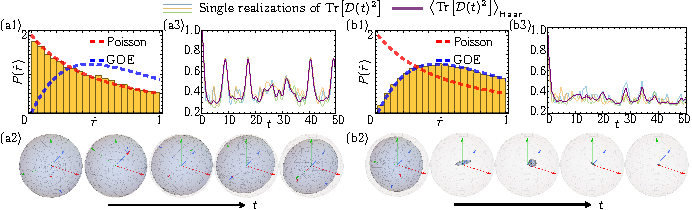
\includegraphics[width=\linewidth]{tikz/cj_purity.pdf}
\DIFaddendFL \caption{Spectral and single-spin dynamical behavior in regular and chaotic regimes of the mixed-field Ising model [\Eref{eq:H:ising}]. Panel (a) corresponds to \DIFdelbeginFL \DIFdelFL{an integrable }\DIFdelendFL \DIFaddbeginFL \DIFaddFL{a regular }\DIFaddendFL regime [$(h_z, J) = (1.446, 0.05)$] and \DIFdelbeginFL \DIFdelFL{the }\DIFdelendFL panel (b) to a chaotic regime [$(h_z, J) = (0.48, 0.8)$], with fixed $h_x=1$. \textbf{(a1), (b1)} Distribution of nearest-neighbor level spacing ratios $P(\tilde{r})$ for $L=16$ (even sector), compared to Poisson (red dashed) and GOE (blue dashed) predictions. \textbf{(a2), (b2)} Action of the quantum channel $\mcE_t$ on the Bloch sphere of the probe spin ($L=7$). The \DIFaddbeginFL \DIFaddFL{solid arrows represent the initial Cartesian axes of the Bloch sphere ($x, y, z$), while the dotted arrows indicate their transformed orientation at later times. In the }\DIFaddendFL chaotic \DIFaddbeginFL \DIFaddFL{regime, the quantum }\DIFaddendFL channel induces a rapid contraction of the sphere volume, contrasting with the coherent precession in the regular case. \textbf{(a3), (b3)} Time evolution of the Choi echo $\Tr[\mcD(t)^2]$ ($L=7$). Low-opacity lines represent single realizations with random initial product states of the environment; the thick purple line corresponds to the analytical Haar-averaged Choi echo $\mathbb{E}[\Tr[\mathcal{D}^{2}(t)]]$ derived in Eq.~\eqref{eq:haar:avg:choi}.}
\label{fig:cj:purity}
\end{figure*}
%DIF < }}
%DIF < 
%DIF <  III. The Choi echo: operational interpretation of the Choi purity{
\DIFaddbegin 


\DIFaddend \section{The Choi echo: operational interpretation of the Choi purity}\label{sec:interpretation}
% Intro of the section: Establishing the thesis (General context)
We now establish an operational interpretation of the Choi purity [cf.~Eq.~\eqref{eq:choi:purity}] by showing that it plays the role of an echo quantifying recoverability under local loss of information. In this formulation, the Choi purity is not merely a static functional of the channel, but a probe of dynamical reversibility analogous in structure to an echo protocol. This perspective highlights its ability to diagnose how strongly the global evolution becomes irreversibly correlated with degrees of freedom that are inaccessible to the subsystem.

%DIF <  Loshmidt echo, definition and context (Broad context)
The Loschmidt echo is a fundamental tool for characterizing the stability of quantum evolution, widely employed in contexts ranging from decoherence theory to critical many-body phenomena~\cite{peres_1984_stability,gorin_2006_dynamics}. 
Defined as $L(t) = |\langle \psi_0 | e^{i (H+\Sigma) t} e^{-i H t} | \psi_0 \rangle|^2$, it quantifies the ability of a system to recover its initial state after a forward evolution \DIFaddbegin \DIFadd{under the reference Hamiltonian }\DIFaddend $H$ \DIFdelbegin \DIFdel{, a perturbation $\Sigma$, and }\DIFdelend \DIFaddbegin \DIFadd{followed by }\DIFaddend a backward evolution \DIFaddbegin \DIFadd{governed by the perturbed Hamiltonian $H + \Sigma$}\DIFaddend .
Its decay reflects the system’s sensitivity to perturbations and serves as a canonical measure of dynamical irreversibility.

%DIF <  Equation of the Choi purity for our novel operational interpretation
In contrast to perturbations of the Hamiltonian, the Choi purity  $\Tr[\mcD(t)^2]$ acts as an echo that probes the stability of the global evolution against a \textit{local} loss of information. Consider the channel $\mathcal{E}_t$ induced by the joint unitary $U(t)$ acting on the initially uncorrelated state $\rho_S\otimes\rho_E$, with $\rho_E=\dyad{\psi}$ any pure state. Combining the Choi definition in \Eref{eq:choi_def} with the system–environment representation of the channel in \Eref{eq:channel_def}, the purity of the Choi state can be recast in the form
\begin{equation}\label{eq:choi_as_le}
\Tr(\mcD^2) = \Bigg\langle\psi\Bigg|
\Tr_S\Bigg[
U^\dagger \Lambda_S \bqty{
U \pqty{\frac{\mathbb{I}_S}{d_S} \otimes \dyad{\psi} } U^\dagger
} U
\Bigg]
\Bigg|\psi\Bigg\rangle.
\end{equation}
Here, $\Lambda_S(\cdot) = (\mathbb{I}_S/d_S)\Tr_S(\cdot)$ represents the completely depolarizing channel acting locally on the subsystem $S$. 
%DIF <  \mgnote{it's not completely obvious to me that is the depolarizing channel}
%DIF <  \janote{Propongo que lo dejemos así. Es un detalle más de las cuentas matemáticas y, más importante, lo dejamos para que un árbitro lo pregunte}
For compactness, we have suppressed the explicit time arguments in this expression, denoting $U \equiv U(t)$ and $\mcD \equiv \mcD(t)$.

% Operational meaning of the Choi purity and discussion
Equation~\eqref{eq:choi_as_le} shows that $\operatorname{Tr}[\mathcal{D}(t)^2]$ is the fidelity with which the environment returns to its initial state after a three-step protocol:  
\begin{enumerate}
\item A forward evolution under $U$, starting from a product state in which $S$ carries no information,
\item A local ``perturbation'' is applied via a completely depolarizing channel $\Lambda_S$, on the system $S$ only, that breaks all entanglement between $S$ and $E$ acquired during the forward evolution.
\item A backward evolution under $U^\dagger$.
\end{enumerate}
The Choi purity therefore quantifies the recoverability of the environment following the loss of subsystem information and plays the role of an \textit{echo}. In consequence, we refer to this quantity as the \textit{Choi echo}.

%DIF <  Because the Choi state is a basis-independent representation of the channel, the Choi echo characterizes reversibility at the level of the reduced dynamics, not of a particular system–environment decomposition. A high echo fidelity indicates that the forward evolution generated only weak non-local correlations, allowing the global state to be reversed even after the subsystem is depolarized. A decaying echo reveals dynamical irreversibility: correlations between $S$ and $E$ have become sufficiently complex that severing them at the subsystem destroys the ability to reconstruct the global state.
\DIFdelbegin %DIFDELCMD < 

%DIFDELCMD < %%%
%DIF <  % Broader Context and Relevance (General applicability)
%DIF <  This operational perspective positions the Choi echo as a tool for diagnosing irreversibility and information scrambling in many-body systems. Unlike entropy-based indicators, which quantify locally inaccessible information, or out-of-time-ordered correlators (OTOCs), which probe operator growth, the Choi echo directly measures the recoverability of global dynamics in the presence of local information loss. Its reliance on the channel alone makes it broadly applicable across contexts ranging from thermalization and localization to signatures of quantum chaos in interacting systems.
%DIFDELCMD < 

%DIFDELCMD < %%%
%DIF <  \mgnote{
\DIFdelend Since the Choi state provides a basis-independent representation of the channel, the Choi echo quantifies reversibility at the level of the reduced dynamics. A high echo fidelity signifies that the forward evolution has generated only weak non-local correlations, so that the global state remains recoverable even after the subsystem has been depolarized. Conversely, a decaying echo signals dynamical irreversibility: correlations between \(S\) and \(E\) have become sufficiently intricate that severing them at the subsystem level eliminates the possibility of reconstructing the global state. This operational viewpoint identifies the Choi echo as a tool for diagnosing irreversibility and information scrambling in many-body systems. In parallel to entropy-based indicators, which quantify locally inaccessible information, and out-of-time-ordered correlators (OTOCs), which probe operator growth, the Choi echo provides a direct measure of the recoverability of global dynamics in the presence of local information loss.
%DIF <  }


%DIF < }
%DIF < 
%DIF <  IV. Choi echo as a local probe{
\section{The Choi echo as a probe for quantum chaos}\label{sec:chaos_probe}
%DIF <  \janote{Para referencia: Aquí hay cosas comentadas}
%DIF < {\color{jacolor}
%DIF < % Establecer el contexto general y la importancia
%DIF < % fundamental de detectar el caos cuántico de muchos cuerpos.
%DIF < The characterization of quantum chaos in many-body systems is a
%DIF < fundamental pursuit that bridges quantum mechanics and statistical
%DIF < mechanics~\cite{bohigas_1984_characterization, deutsch_1991_quantum, srednicki_1994_chaos, rigol_2008_thermalization}.
%DIF < The onset of chaos is intrinsically linked to
%DIF < the mechanism of thermalization in isolated quantum systems, as
%DIF < formalized by the Eigenstate Thermalization Hypothesis (ETH)~\cite{dalessio_2016_quantum, deutsch_1991_quantum, srednicki_1994_chaos}.
%DIF < Understanding this connection is critical for topics ranging from
%DIF < many-body localization
%DIF < (MBL)~\cite{nandkishore_2015_manybody, abanin_2019_colloquium, pal_2010_manybody} and the scrambling of quantum
%DIF < information~\cite{shenker_2014_black, maldacena_2016_bound, swingle_2018_unscrambling, xu_2020_does} to the dynamics of black
%DIF < holes~\cite{maldacena_2016_bound, balasubramanian_2025_quantum} and
%DIF < the stability of quantum computation~\cite{georgeot_2000_emergence, c_2025_disordering}.
%DIF < 
%DIF < % Introducir el "gold standard" (RMT / la r) y su
%DIF < % limitación computacional y experimental fundamental.
%DIF < The canonical diagnostic for quantum chaos is rooted in random
%DIF < matrix theory (RMT)~\cite{bohigas_1984_characterization, mehta_2004_random}. The spectral statistics of chaotic
%DIF < Hamiltonians exhibit level repulsion, mirroring the predictions of
%DIF < RMT, while integrable systems display uncorrelated level spacings
%DIF < described by a Poisson distribution~\cite{berry_1977_level, akhshani_2025_statistical}. In modern practice,
%DIF < this is robustly quantified by the mean level spacing ratio,
%DIF < $\langle \tilde{r} \rangle$~\cite{oganesyan_2007_localization, atas_2013_distribution}, which avoids the complexities
%DIF < of spectral unfolding~\cite{oganesyan_2007_localization}. However, calculating $\langle
%DIF < \tilde{r} \rangle$ requires \cdnote*{o the entire knowledge of the spectrum, ESTILO}{\color{blue}full exact diagonalization}\janote{de acuerdo, la propuesta de Charly incluye el POV experimental. Cambio:}
%DIF < However, calculating $\ev{r}$ requires access to the full spectrum, 
%DIF < a task that grows computationally and experimentally intractable with 
%DIF < increasing system size for typical many-body systems.~\cite{scialchi_2024_integrabilitytochaos}. This diagnostic is also inaccessible in experimental
%DIF < platforms, such as ion traps or cold atoms, which are designed to
%DIF < probe dynamics rather than the full energy spectrum~\cite{das_2025_proposal, vallejo-fabila_2025_singlesite}.
%DIF < \mgnote{This paragraph could be the initial one, specially the $\langle
%DIF < \tilde{r} \rangle$ discussion, which motivates the introduction of local probes.}
%DIF < 
%DIF < % Introducir la hipótesis del "proxy" (dinámica local,
%DIF < % \statep) y los trabajos que la han validado.
%DIF < This limitation motivates an intensive search for simpler,
%DIF < computationally feasible, and experimentally accessible dynamical
%DIF < proxies for quantum chaos~\cite{das_2025_proposal, scialchi_2024_integrabilitytochaos, c_2025_disordering}. 
%DIF < A central hypothesis has emerged, suggesting that the dynamics of a local 
%DIF < subsystem can serve as a faithful indicator of \janote{\sout{global,}} many-body chaos~\cite{dalessio_2016_quantum, borgonovi_2025_timescales}. A
%DIF < prominent candidate is the averaged subsystem state purity,
%DIF < $\overline{\mathcal{P}}$, which quantifies the equilibration of a
%DIF < single probe spin coupled to the rest of the chain. Recent work
%DIF < demonstrated a strong anti-correlation between $\overline{\mathcal{P}}$
%DIF < and $\langle \tilde{r} \rangle$ across several spin models, seemingly
%DIF < validating single-spin decoherence as a reliable proxy for the
%DIF < integrability-to-chaos transition~\cite{mirkin_2021_quantum}.
%DIF < 
%DIF < %promediado sobre estados iniciales
%DIF < The quantum channel $\mcE_t$, as defined in \Eref{eq:channel_def}, depends
%DIF < explicitly on both the unitary evolution $U(t)$ and the initial
%DIF < environment state $\rho_E$. In our setup, the evolution is governed
%DIF < by the Hamiltonian $H$ via $U(t) = e^{-iHt}$. We aim to
%DIF < characterize the generic dynamical properties encoded in $H$---which
%DIF < determines the system's chaotic or integrable nature---rather than
%DIF < properties tied to a specific initial state $\rho_E$.
%DIF < We therefore average over an ensemble of initial environment
%DIF < states. This procedure ensures our final indicator depends only on the
%DIF < statistical properties of the chosen ensemble, not on any particular member.
%DIF < Specifically, we consider pure product states of the form
%DIF < $\rho_E = \bigotimes_{j \in E} \dyad{\psi_j}$, where each spin state
%DIF < $\ket{\psi_j}$ is drawn independently from the Haar measure.
%DIF < This ensemble average corresponds to an infinite-temperature condition~\footnote{\janote{When averaged over the Haar measure, a single spin state $\dyad{\psi_j}$ becomes the maximally mixed state $\mathbb{I}/2$. The full environment state $\rho_E$, being a tensor product of $L-1$ such states, thus averages to $\langle \rho_E \rangle = \mathbb{I}_E / 2^{L-1}$, which is the state of infinite-temperature equilibrium.}},
%DIF < ensuring that the dynamics samples the entire energy spectrum. 
%DIF < 
%DIF < % Declarar la metodología del benchmark y el resultado
%DIF < % principal de que la correspondencia falla.
%DIF < We perform a systematic benchmark of all three indicators---the
%DIF < spectral $\mlsr$, the state purity $\statep$, and our channel purity
%DIF < $\choip$---across the regular-to-chaos transition. We employ
%DIF < three paradigmatic one-dimensional spin-1/2 chain models: the
%DIF < mixed-field Ising model~\cite{kim_2014_testing, borgonovi_2016_quantum}, the Heisenberg model with random
%DIF < fields~\cite{oganesyan_2007_localization, luitz_2015_manybody}, and the XXZ model with a local defect~\cite{santos_2004_integrability, brenes_2018_hightemperature}. We compute this ensemble average analytically, as detailed
%DIF < in Appendix~\ref{app:haar}, yielding
%DIF < \begin{widetext}
%DIF < \begin{equation}\label{eq:haar:avg:choi}
%DIF < \mathbb{E}\Big[\Tr\bqty{\mathcal{D}^{2}(t)}\Big] 
%DIF < = 
%DIF < \frac{1}{12^{L-1}} \sum_{\vec{\alpha} \in \{0,x,y,z\}^{L-1}}
%DIF <   3^{\frac{1}{2}\qty(L - 1 - w(\vec{\alpha}))}
%DIF < \Tr \Big[ \Tr_S^2 \big[U(t)
%DIF < \qty(\sigma_1^0 \sigma_2^{\alpha_2} \ldots \sigma_L^{\alpha_L})
%DIF < U^\dagger(t) \big] \Big] \, ,
%DIF < \end{equation}
%DIF < \end{widetext}
%DIF < where $\vec{\alpha} = (\alpha_2, \dots, \alpha_L)$ is a vector of Pauli
%DIF < indices from the set $\{0,x,y,z\}^{L-1}$, $\sigma_j^0$ is the
%DIF < identity operator on the spin $j$, and $w(\vec{\alpha})$ counts the
%DIF < number of non-identity operators ($\alpha_i \neq 0$) in the
%DIF < environment's tensor product. \janote{Me acabo de dar cuenta que traza de la pureza de Choi debe poderse promediar sobre un entorno de máximo $d_E=4$. Quizás lo podemos poner como curiosidad o trabajo futuro} \mgnote{A mi si me interesa eso.}
%DIF < The result of this average, $\mathbb{E}[\Tr[\mathcal{D}^{2}(t)]]$,
%DIF < is plotted as the thick purple lines in
%DIF < Figs.~\ref{fig:cj:purity}(a3) and \ref{fig:cj:purity}(b3).
%DIF < This curve provides a representative measure of the dynamics
%DIF < induced by $H$, averaged over the initial environmental
%DIF < configurations.
%DIF < }

%DIF <  Mini intro and context of quantum chaos
\DIFdelbegin \DIFdel{The characterization of }\DIFdelend \DIFaddbegin \DIFadd{Diagnosing the transition to }\DIFaddend quantum chaos in many-body systems \DIFdelbegin \DIFdel{is central to understanding thermalization, information scrambling, and the emergence of statistical mechanics from unitary }\DIFdelend \DIFaddbegin \DIFadd{typically relies on identifying statistical fingerprints within both the energy spectrum and the system's }\DIFaddend dynamics~\cite{dalessio_2016_quantum}. Quantum-chaotic behavior manifests itself through several universal features: (i) spectral statistics governed by Random Matrix Theory (RMT)~\cite{bohigas_1984_characterization}, (ii) eigenstate properties consistent with the eigenstate thermalization hypothesis (ETH)~\cite{deutsch_1991_quantum}, and (iii) extreme sensitivity to perturbations, captured by Loschmidt echoes and out-of-time-ordered correlators (OTOCs). These signatures reflect distinct facets of the same phenomenon—namely, the progressive spreading of quantum information over the many-body Hilbert space. 
In practice, however, diagnosing chaos is challenging: spectral probes require access to the \DIFdelbegin \DIFdel{dense interior }\DIFdelend \DIFaddbegin \DIFadd{bulk }\DIFaddend of the spectrum, while OTOCs and echo protocols demand controlled perturbations and precise reversals~\cite{bardarson2012unbounded,santos2010onset,alba2017entanglement,smith2016many}.
This motivates the development of diagnostics that are more computationally tractable and physically accessible.

%DIF <  The spectral metric: Mean Level Spacing Ratio
Focusing first on spectral indicators, chaotic systems display level repulsion consistent with RMT, whereas integrable models exhibit the uncorrelated spectrum characteristic of Poisson statistics~\cite{berry_1977_level}. \DIFaddbegin \DIFadd{In this work, we use the term ``integrable'' to encompass both exactly solvable systems (e.g., via the Bethe ansatz) and systems that effectively display Poissonian spectral statistics due to finite-size effects~}\protect\footnote{\DIFadd{A rigorous definition of many-body quantum integrability requires the thermodynamic limit~\mbox{%DIFAUXCMD
\cite{caux_2011_remarks}}\hskip0pt%DIFAUXCMD
. For instance, the mixed-field Ising model used in this work has been formally shown to be non-integrable for any non-zero $J$~\mbox{%DIFAUXCMD
\cite{chiba_2024_proof}}\hskip0pt%DIFAUXCMD
.}}\DIFadd{. }\DIFaddend A robust measure of these short-range correlations is the mean level spacing ratio $\langle \tilde{r} \rangle$, defined as the average of $\tilde{r}_n = \min(s_n, s_{n-1})/\max(s_n, s_{n-1})$ for consecutive spacings $s_n = E_{n+1} - E_n$, evaluated within a fixed symmetry sector~\cite{oganesyan_2007_localization}. As illustrated in Figs.~\ref{fig:cj:purity}(a1) and (b1) for the mixed-field Ising chain [cf.~Eq.~\eqref{eq:H:ising}], the empirical distribution shifts from the Poissonian form,
\(
P_{\text{P}}(\tilde{r}) = 2/(1+\tilde{r})^2,
\)
to the Wigner-Dyson surmise characteristic of the Gaussian Orthogonal Ensemble (GOE),
\(
P_{\text{GOE}}(\tilde{r}) = 8(\tilde{r} + \tilde{r}^2) / [7(1+\tilde{r}+\tilde{r}^2)^{5/2}],
\)\DIFaddbegin \DIFadd{~\mbox{%DIFAUXCMD
\cite{atas_2013_distribution}}\hskip0pt%DIFAUXCMD
, }\DIFaddend marking the transition from integrable to chaotic behavior\DIFdelbegin \DIFdel{~\mbox{%DIFAUXCMD
\cite{atas_2013_distribution}}\hskip0pt%DIFAUXCMD
}\DIFdelend . Although higher-order ratios mitigate the need for explicit desymmetrization~\cite{tekur_2020_symmetry}, all spectral probes fundamentally require resolving large portions of the many-body spectrum, a task that becomes prohibitive for large Hilbert spaces~\DIFdelbegin \DIFdel{\mbox{%DIFAUXCMD
\cite{scialchi_2024_integrabilitytochaos, bernien2017probing, huang2020predicting, brydges2019probing}}\hskip0pt%DIFAUXCMD
}\DIFdelend \DIFaddbegin \DIFadd{\mbox{%DIFAUXCMD
\cite{scialchi_2024_integrabilitytochaos, bernien2017probing, huang_2020_predicting, brydges2019probing}}\hskip0pt%DIFAUXCMD
}\DIFaddend .

%DIF <  State purity of reduced subsystems as local probe for the onset of quantum chaos
These limitations have motivated the search for accessible dynamical probes. Under chaotic dynamics, canonical typicality implies that small subsystems equilibrate toward stationary states that depend only on global conserved quantities~\cite{goldstein_2006_canonical, rigol_2008_thermalization}. In the context of spin chains, the degree of equilibration of a single probe spin---typically identified with the first site of the chain---has been shown to correlate strongly with spectral signatures of chaos of the entire many-body system~\cite{mirkin_2021_quantum}. Quantitatively, this is captured by the averaged subsystem purity,
\begin{equation}\label{eq:avg:P}
\overline{\mathcal{P}}=\frac{1}{N}\sum_{i=1}^N
\left(\frac{1}{T}\int_0^T \Tr[\rho_{S,i}^2(t)]\,dt\right),
\end{equation}
computed over $N$ random initial product states and a time window $[0,T]$. Across diverse spin models, $\overline{\mathcal{P}}$ exhibits a strong anticorrelation with $\langle \tilde{r} \rangle$, suggesting that \DIFdelbegin \DIFdel{local }\DIFdelend \DIFaddbegin \DIFadd{single-spin }\DIFaddend decoherence can serve as an experimentally friendly probe of the integrability-to-chaos transition.

However, a fundamental question remains: does \DIFdelbegin \DIFdel{local }\DIFdelend \DIFaddbegin \DIFadd{single-spin }\DIFaddend decoherence provide an unambiguous signature of many-body chaos, or can integrable dynamics produce similar behavior through mechanisms such as coherent transport? To address this, we employ the Choi echo framework introduced in Sec.~\ref{sec:interpretation}, applied to one-dimensional spin-$1/2$ chains of length $L$. We partition the system such that the first spin acts as the probe $S$, while the remaining $L-1$ spins form the environment $E$. The probe’s reduced dynamics are encoded in the quantum channel $\mathcal{E}_t$ generated by the global unitary $U(t)=e^{-iHt}$ [cf.~Eq.~\eqref{eq:channel_def}]. As shown in Figs.~\ref{fig:cj:purity}(a2) and (b2), integrable evolution preserves a coherent Bloch-sphere trajectory, whereas chaotic evolution induces a rapid contraction of the Bloch volume, signaling strong decoherence. Unlike state purity, which depends on the specific initial condition, the Choi echo $\Tr[\mathcal{D}(t)^2]$ probes the intrinsic reversibility of the channel itself. By quantifying the stability of global correlations against a depolarizing operation on the probe, it provides a stricter and state-independent diagnostic of decoherence.

To isolate the generic dynamical properties of the Hamiltonian $H$ from specific initial states of the environment, we compute the analytical Haar average of the Choi echo over product states of the environment. Each environmental spin state is drawn independently from the Haar measure, a procedure corresponding to an infinite-temperature average~\footnote{When averaged over the Haar measure, a \DIFdelbegin \DIFdel{single spin }\DIFdelend \DIFaddbegin \DIFadd{single-spin }\DIFaddend state $\dyad{\psi_j}$ becomes the maximally mixed state $\mathbb{I}/2$. The full environment state $\rho_E$, being a tensor product of $L-1$ such states, thus averages to $\langle \rho_E \rangle = \mathbb{I}_E / 2^{L-1}$, which is the state of infinite-temperature equilibrium.}. As derived in Appendix~\ref{app:haar}, this yields:
\begin{align}\label{eq:haar:avg:choi}
\mathbb{E}\bqty{\Tr\pqty{\mathcal{D}^{2}}} =& 
% \frac{1}{4^{L-1}} 
\sum_{\vec{\alpha} }
%DIF <  \in \{0,x,y,z\}^{L-1}}
  %DIF >  \in \{0,x,y,z\}^{L-1}
  \frac{4^{-L}}{3^{w(\vec{\alpha})}}
\Tr \Big[ \Tr_S^2 \big[U
\qty(\sigma_1^0 \sigma_2^{\alpha_2} \ldots \sigma_L^{\alpha_L})
U^\dagger \big] \Big],
\end{align}
where $\vec{\alpha} \in \{0,x,y,z\}^{L-1}$, and for compactness we have  suppressed the explicit time dependence. Here $\sigma_j^\mu$ denotes the Pauli 
operator labeled by $\mu \in \{0,x,y,z\}$ acting on site $j$ (with $\sigma^0 \equiv \mathbb{I}$), 
and $w(\vec{\alpha})$ counts the number of non-identity operators in the 
environment string $\vec{\alpha} = (\alpha_2, \dots, \alpha_L)$. This analytical average is depicted in Figs.~\ref{fig:cj:purity}(a3) and (b3), where the Haar-averaged Choi echo (thick line) effectively filters out the fluctuations inherent to single environment realizations (low-opacity lines). To construct a direct analogue of $\langle \tilde{r} \rangle$ and $\overline{\mathcal{P}}$, we also average in time the Haar-averaged Choi echo:
\DIFaddbegin 

\DIFaddend \begin{equation}\label{eq:avg:CJ}
\expval{\Tr[\mcD(t)^2]}\DIFdelbegin \DIFdel{_{\text{Haar}, t} }\DIFdelend \DIFaddbegin \DIFadd{_{\text{Haar}, T} }\DIFaddend = \frac{1}{T}
\int_{0}^{T} \mathbb{E}\Big[\Tr[\mathcal{D}^{2}(t)]\Big] \, dt.
\end{equation}
\DIFaddbegin 

\DIFaddend The next section compares $\langle \tilde{r} \rangle$, $\overline{\mathcal{P}}$, and the Haar-averaged Choi echo across different models and parameter regimes.
%DIF < }
%DIF < 
%DIF <  V. Model Systems and Numerical Analysis{
\DIFaddbegin 


\DIFaddend \section{Model Systems and Numerical Analysis}\label{sec:models_results}

We now assess the performance of the Choi echo as a dynamical probe for the transition to quantum chaos. To this end, we analyze three paradigmatic one-dimensional spin-$1/2$ models that exemplify distinct mechanisms of integrability breaking—competing fields, quenched disorder, and local defects. This diversity provides a stringent test of whether the echo can meaningfully separate chaotic from non-chaotic dynamics using \DIFdelbegin \DIFdel{only local information }\DIFdelend \DIFaddbegin \DIFadd{information only from single-spin dynamics}\DIFaddend .

\subsection{Spin Chain Hamiltonians}\label{sec:spin_chains}

%DIF <  Fig 2, mapas ising{
\begin{figure*}
\DIFdelbeginFL %DIFDELCMD < 
\includegraphics[width=\textwidth]{figures/ising.pdf}
%DIFDELCMD < %%%
\DIFdelendFL \DIFaddbeginFL 
\includegraphics[width=\textwidth]{tikz/ising.pdf}
\DIFaddendFL \caption{Comparison of short-range spectral statistics and \DIFdelbeginFL \DIFdelFL{local }\DIFdelendFL \DIFaddbeginFL \DIFaddFL{single-spin }\DIFaddendFL dynamical probes for the mixed-field Ising model [\Eref{eq:H:ising}] as a function of $h_z/h_x$ and $J/h_x$. \textbf{(a)} Mean level spacing ratio $\langle \tilde{r} \rangle$, computed for $L = 16$ within the even symmetric sector. \textbf{(b)}, \textbf{(c)} \DIFdelbeginFL \DIFdelFL{Local }\DIFdelendFL \DIFaddbeginFL \DIFaddFL{Single-spin }\DIFaddendFL dynamical probes computed for the spin at the first site ($L = 7$): \textbf{(b)} averaged subsystem state purity $\statep$ [\Eref{eq:avg:P}] ($N=50$, $T=100$); \textbf{(c)} averaged Choi echo $\choip$ [\Eref{eq:avg:CJ}] ($T=100$). The horizontal red dashed line ($J/h_x=1$) indicates the parameter cut where the correspondence between $\mlsr$ and $\statep$ was analyzed in Ref.~\cite{mirkin_2021_quantum} for $h_z/h_x \in [0, 2.5]$.}
\label{fig:cj:purity:ising}
\end{figure*}
%DIF < }

\subsubsection{Mixed-field Ising model}\label{sec:ising}
We first consider the mixed-field Ising model with open boundary conditions, described by the Hamiltonian:
\begin{equation}\label{eq:H:ising}
H = \sum_{i=1}^L \left( h_x \sigma_i^x + h_z \sigma_i^z \right) - J \sum_{i=1}^{L-1} \sigma_i^z \sigma_{i+1}^z \, ,
\end{equation}
where $\sigma_i^\alpha$ ($\alpha \in \{x,y,z\}$) are Pauli operators, $L$ is the chain length, $J$ is the nearest-neighbor Ising interaction, and $h_x, h_z$ are transverse and longitudinal field strengths. This model possesses a global spatial reflection symmetry $\mathcal{R}$ ($i \leftrightarrow L-i+1$), decomposing the Hilbert space into even and odd parity sectors. The model is integrable in two limits: the transverse-field Ising model ($h_z = 0$), solvable via Jordan-Wigner transformation~\cite{sachdev_2011_quantum}, and the so-called classical Ising model ($h_x = 0$)~\cite{baxter_2007_exactly}. When $J=0$, the system decouples into a non-interacting set of $L$ spins. The simultaneous presence of all three terms breaks integrability, rendering it a standard testbed for quantum chaos~\cite{kim_2014_testing,garrison_2018_does,borgonovi_2016_quantum}. Notably, it has been rigorously proven that for any non-zero $J$, $h_x$, and $h_z$, the model possesses no non-trivial local conserved quantities~\cite{chiba_2024_proof}. The chaotic regime is frequently studied using parameters where all three terms are of comparable magnitude, $J \sim h_x \sim h_z$, as this maximizes the non-commutation responsible for driving chaotic behavior~\cite{karthik_2007_entanglement,atas_2017_quantum,camargo_2024_spread}.


\subsubsection{Heisenberg model with random fields}\label{sec:heisenberg}
Next, we examine the Heisenberg model with random fields:
\begin{equation}\label{eq:H:heisenberg}
H = \frac{1}{4}\sum_{i=1}^{L-1} \left(\vec{\sigma}_i \cdot \vec{\sigma}_{i+1}\right) + \frac{1}{2}\sum_{i=1}^L h_i \sigma_i^z \, ,
\end{equation}
where $h_i$ are independent random variables drawn uniformly from the interval $[-h, h]$, and $h$ denotes the disorder strength. This model conserves the total magnetization $M_z = \sum_i \sigma_i^z$. This $U(1)$ symmetry is equivalent to conserving the total number of up spins, $N_{\uparrow}$, related to the magnetization via $\ev{M_z} = 2N_{\uparrow} - L$. The clean limit ($h=0$) is integrable by Bethe-anzats~\cite{bethe_1931_zur}. For $h>0$, integrability is broken. This Hamiltonian describes the transition from an ergodic or thermal phase ($h \lesssim 3.5$) to a many-body localized (MBL) phase at strong disorder~\cite{oganesyan_2007_localization,luitz_2015_manybody,abanin_2019_colloquium}.

\subsubsection{XXZ model with a local defect}\label{sec:xxz}
Finally, we study the XXZ model with a single local defect:
\begin{equation}\label{eq:H:xxz}
H = \frac{1}{4}\sum_{i=1}^{L-1} \left[ J_{xy} (\sigma_i^x\sigma_{i+1}^x + \sigma_i^y\sigma_{i+1}^y) + J_z \sigma_i^z\sigma_{i+1}^z \right] + \frac{1}{2}\varepsilon \sigma_d^z \, .
\end{equation}
Here, $J_{xy}$ and $J_z$ are anisotropic interaction strengths, and $\varepsilon$ is the field strength at a defect site $d$. Like the Heisenberg model, this system conserves $M_z$. The defect is placed near the center to break spatial reflection symmetry explicitly. For $\varepsilon = 0$, the model is integrable~\cite{bethe_1931_zur}. A non-zero defect $\varepsilon \neq 0$ breaks integrability~\cite{santos_2004_integrability,brenes_2018_hightemperature,pandey_2020_adiabatic}, providing a minimal model where chaos is induced solely by a local perturbation on a single site. We note that in the limit $\varepsilon \gg 1$, the chain effectively decouples into two non-interacting parts.


\subsection{Results}\label{sec:results_discussion}
%DIF <  We benchmark the averaged Choi echo, $\expval{\Tr[\mcD^2]}_{\text{Haar},t}$ (denoted hereafter as $\choip$), against the averaged subsystem state purity $\statep$ and the mean level spacing ratio $\expval{\tilde{r}}$. Both purities are computed for the probe spin at the first site ($i=1$).
\DIFdelbegin %DIFDELCMD < 

%DIFDELCMD < %%%
%DIF <  The subsystem purity $\statep$ [Eq.~\eqref{eq:avg:P}] is computed by averaging over $N=50$ random product initial states and a time interval $[0, T]$ with $T = 100$. Similarly, the Choi echo $\choip$ [Eq.~\eqref{eq:avg:CJ}] is time-averaged over the same interval, evaluating the Haar average analytically via Eq.~\eqref{eq:haar:avg:choi}. We verified that the intensity maps remain qualitatively invariant for system sizes $3 \le L \le 7$ (data for $L < 7$ not shown). Consequently, given this robustness and the exponential cost of evaluating the $4^L$ terms in Eq.~\eqref{eq:haar:avg:choi} at every time step, we present results for $L=7$. This choice is further justified physically by the nearest-neighbor nature of the interactions in our models. Since the probe spin couples directly only to its immediate neighbor, the local energy scale and the mechanism initiating information outflow are independent of the total chain length. In contrast, to ensure robust spectral statistics, $\expval{\tilde{r}}$ is computed via exact diagonalization for larger systems ($L=16$ or $L=18$) within specific symmetry sectors. This difference in system sizes imposes a stringent test on the dynamical probes: can they predict the same transition to quantum chaos using only a local observation?
%DIFDELCMD < 

%DIFDELCMD < %%%
\DIFdelend We benchmark the Haar- and time-averaged Choi echo $\choip$ [Eq.~\eqref{eq:avg:CJ}] against two reference indicators:  
(i) the averaged subsystem state purity $\statep$ [Eq.~\eqref{eq:avg:P}], and  
(ii) the mean level spacing ratio $\langle \tilde{r} \rangle$, which provides the spectral ground for quantum many-body chaos. While both purities are computed for small chains ($L=7$) with the probe at site $1$, the spectral statistics are evaluated via exact diagonalization on significantly larger systems ($L=16$ or $L=18$). This mismatch in system sizes imposes a stringent requirement: a reliable \DIFdelbegin \DIFdel{local }\DIFdelend \DIFaddbegin \DIFadd{single-spin }\DIFaddend dynamical probe must be robust to finite-size effects and must recover the chaotic transition inferred from the spectral benchmark.

%DIF <  Ising
\subsubsection{Resolving chaos and decoupling in the mixed-field Ising model}
% Presentar detalles cálculos y comentar que la resolución es mejor con el echo de Choi
\Fref{fig:cj:purity:ising} compares the three quantities across the $(J/h_x,\,h_z/h_x)$ plane. The mean level spacing ratio is computed for $L=16$ within the even sector (dimension 32,898). As shown in Fig.~\ref{fig:cj:purity:ising}(a), it exhibits a well-defined chaotic dome where $\langle \tilde{r} \rangle \approx 0.53$. Despite the reduced system size, both $\statep$ and $\choip$ reproduce this structure, with low purity correlating with high $\langle \tilde{r} \rangle$. Notably, the Choi echo [Fig.~\ref{fig:cj:purity:ising}(c)] resolves the boundaries of the chaotic region more sharply than the state purity [Fig.~\ref{fig:cj:purity:ising}(b)].

% Comentar sobre la discrepancia (gradiente en las purezas) 
However, a discrepancy emerges in the regular region $1.5 \le h_z/h_x \le 3$ under weak coupling $J/h_x < 0.5$, indicating that the dynamical probes do not anticorrelate with the spectral statistics across the full parameter space. In this regime, the mean level spacing ratio $\mlsr$ saturates at its Poisson value ($\approx 0.38$), whereas both dynamical probes display a smooth gradient. As $J/h_x$ decreases, the Choi echo and the state purity increase gradually, reaching their maxima only when $J \to 0$. Thus, while spectral statistics detect a uniform regular phase, \DIFdelbegin \DIFdel{local }\DIFdelend \DIFaddbegin \DIFadd{single-spin }\DIFaddend probes remain sensitive to the competition between the Ising coupling $J$ and the local fields $(h_x, h_z)$. The Choi echo, in particular, captures the continuous drift toward locally unitary dynamics as interactions become negligible.

% Comentar donde sí el echo de Choi se anticorrelaciona y comparación con trabajo de Wisniacki 
Finally, in regions where the interaction $J$ is comparable to the local fields, \DIFdelbegin \DIFdel{local }\DIFdelend \DIFaddbegin \DIFadd{single-spin }\DIFaddend probes regain a faithful anticorrelation with $\mlsr$, as observed along the parameter cut indicated by the red dashed line in Fig.~\ref{fig:cj:purity:ising} ($J/h_x = 1$). This is precisely the regime analyzed in Ref.~\cite{mirkin_2021_quantum} for $0 < h_z/h_x < 2.5$, where both dynamical and spectral indicators show consistent signatures of chaos.



% Case 2: Heisenberg
\subsubsection{Tracking the thermal-to-MBL transition in the Heisenberg model with random fields}

%DIF < fig 3, resultados heisenberg{
\begin{figure}
\DIFdelbeginFL %DIFDELCMD < 
\includegraphics[width=\columnwidth]{figures/heisenberg.pdf}
%DIFDELCMD < %%%
\DIFdelendFL \DIFaddbeginFL 
\includegraphics[width=\columnwidth]{tikz/heisenberg.pdf}
\DIFaddendFL \caption{Comparison of spectral statistics and \DIFdelbeginFL \DIFdelFL{local }\DIFdelendFL \DIFaddbeginFL \DIFaddFL{single-spin }\DIFaddendFL dynamical probes for the Heisenberg model with random fields [\Eref{eq:H:heisenberg}] as a function of disorder strength $h$. All quantities are averaged over 30 disorder realizations. \textbf{Symbols:} Mean level spacing ratio $\langle \tilde{r} \rangle$, computed for $L=18$ within different magnetization sectors $N_{\uparrow}$ (horizontal lines indicate GOE and Poisson limits). \textbf{Solid lines:} \DIFdelbeginFL \DIFdelFL{Local }\DIFdelendFL \DIFaddbeginFL \DIFaddFL{Single-spin }\DIFaddendFL dynamical probes computed for the spin at the first site ($L=7$), plotted as deviations from unity (impurities): \textbf{Left axis (blue):} averaged subsystem state impurity $1-\statep$ [\Eref{eq:avg:P}] ($N=50$, $T=100$); \textbf{Right axis (brown):} averaged Choi echo deviation $1-\choip$ [\Eref{eq:avg:CJ}] ($T=100$). Shaded bands and error bars indicate the standard deviation.}
\label{fig:cj:purity:heisenberg}
\end{figure}
%DIF < }

In the Heisenberg model with random fields, we examine the transition from thermal to the MBL phase. \Fref{fig:cj:purity:heisenberg} displays the spectral and dynamical metrics as a function of disorder strength $h$, with all quantities averaged over 30 disorder realizations. The mean level spacing ratio $\mlsr$ is computed for $L=18$ across five magnetization sectors, specified by the number of up spins $N_{\uparrow} \in \{4, 5, 6, 7, 13\}$, with corresponding Hilbert space dimensions 3,060, 8,568, 18,564, 31,824, and 8,568, respectively. These results, shown as symbols with error bars, capture the crossover from GOE to Poisson statistics around $h_c \approx 3.5$. Here, we observe a robust agreement between the spectral statistics and the \DIFdelbegin \DIFdel{local }\DIFdelend \DIFaddbegin \DIFadd{single-spin }\DIFaddend probes. Both the deviation of the Choi echo from unity ($1-\choip$) and the state impurity ($1-\statep$) remain high in the thermal phase ($h \lesssim 1$) and decay as the system transitions to the MBL phase. Significantly, in the deep thermal phase, the Choi echo exhibits negligible variance across disorder realizations (the standard deviation band in Fig.~\ref{fig:cj:purity:heisenberg} is virtually indiscernible), suggesting it is a stable quantifier of the dynamical map's scrambling power. In contrast, the state purity shows larger fluctuations, reflecting its dependence on the specific initial state trajectory.

% Case 3: XXZ
\subsubsection{Transport-induced false positives for chaos in the XXZ model with a local defect}\label{sec:results_xxz}

Finally, the results for the XXZ model with a local defect reveal a second fundamental limitation of \DIFdelbegin \DIFdel{local }\DIFdelend \DIFaddbegin \DIFadd{the single-spin }\DIFaddend dynamical probes when contrasted with spectral statistics of the full chain. \Fref{fig:cj:purity:xxz} shows intensity maps of $\mlsr$, $\statep$, and $\choip$ as functions of the anisotropy $J_{xy}/J_z$ and defect strength $\varepsilon/J_z$. The spectral benchmark $\mlsr$ [Fig.~\ref{fig:cj:purity:xxz}(a)] is computed for $L=18$ in the $N_{\uparrow}=7$ sector (dimension 31,824), with the defect placed at site $d=9$. The dynamical probes [Figs.~\ref{fig:cj:purity:xxz}(b,c)] are obtained for $L=7$ with the defect at site $d=3$. In both cases, the defect lies in the bulk but away from the reflection axis, ensuring explicit parity breaking. This placement avoids accidental residual symmetries and makes the intensity maps qualitatively comparable despite the different system sizes.

The most prominent discrepancy appears in the region $J_{xy}/J_z > 1$ with a vanishing defect $\varepsilon \to 0$. Here the model approaches the clean XXZ chain and is integrable, a fact captured by $\mlsr$, which saturates at the Poisson value. In sharp contrast, both dynamical probes yield low values that are indistinguishable from the chaotic regime. This constitutes a spurious signature of GOE statistics: strong interactions lead to fast \DIFdelbegin \DIFdel{local }\DIFdelend \DIFaddbegin \DIFadd{single-spin }\DIFaddend relaxation of the probe, overwhelming the global integrable structure and producing a false positive for chaos.

A second, more subtle discrepancy mirrors the behavior observed in the mixed-field Ising model. For $J_{xy}/J_z \lesssim 1$, the spectral indicator $\mlsr$ exhibits a sharp transition toward regular behavior as $J_{xy}$ decreases. The dynamical probes, however, respond through a smooth gradient: as $J_{xy} \to 0$, the flip-flop term responsible for spin transport vanishes and the probe dynamics crosses over continuously to an Ising-type dephasing channel. Thus, while spectral statistics detect the abrupt breakdown of GOE correlations, the \DIFdelbegin \DIFdel{local }\DIFdelend \DIFaddbegin \DIFadd{single-spin }\DIFaddend probes remain sensitive to the gradual suppression of transport rather than the transition to the integrable limit.

%DIF < fig 4, resultados xxz{
\begin{figure*}
\DIFdelbeginFL %DIFDELCMD < 
\includegraphics[width=\textwidth]{figures/xxz.pdf}
%DIFDELCMD < %%%
%DIF < 
\DIFdelendFL \DIFaddbeginFL 
\includegraphics[width=\textwidth]{tikz/xxz.pdf}
\DIFaddendFL \caption{Comparison of spectral statistics and \DIFdelbeginFL \DIFdelFL{local }\DIFdelendFL \DIFaddbeginFL \DIFaddFL{single-spin }\DIFaddendFL dynamical probes for the XXZ model with a local defect [\Eref{eq:H:xxz}] as a function of $J_{xy}/J_z$ and $\varepsilon/J_z$. \textbf{(a)} Mean level spacing ratio $\langle \tilde{r} \rangle$, computed for $L=18$ ($N_{\uparrow}=7$) with the defect at site $d=9$. \textbf{(b)}, \textbf{(c)} \DIFdelbeginFL \DIFdelFL{Local }\DIFdelendFL \DIFaddbeginFL \DIFaddFL{Single-spin }\DIFaddendFL dynamical probes computed for the spin at the first site ($L=7$) with the defect at site $d=3$: \textbf{(b)} averaged subsystem state purity $\statep$ [\Eref{eq:avg:P}] ($N=50$, $T=100$); \textbf{(c)} averaged Choi echo $\choip$ [\Eref{eq:avg:CJ}] ($T=100$). In both configurations, the defect placement explicitly breaks spatial reflection symmetry.}
\label{fig:cj:purity:xxz}
\end{figure*}
%DIF < }
\DIFdelbegin %DIFDELCMD < 

%DIFDELCMD < %%%
%DIF < \subsection{Discussion}% Old discussion
%DIF < Collectively, these results clarify the distinction between \textit{local
%DIF < decoherence} and \textit{quantum chaos}. While chaotic systems generally induce
%DIF < rapid decay of the Choi echo (irreversibility), the converse is not always true. 
%DIF < High decoherence can arise in integrable systems due to strong local 
%DIF < interactions or coherent transport (as seen in the XXZ model with a local 
%DIF < defect). The Choi echo, by probing the reversibility of the channel, confirms 
%DIF < that local probes are sensitive to the \textit{mechanism} of information 
%DIF < loss—whether via quantum chaotic dynamics or transport—whereas spectral statistics are sensitive to the correlations of the spectrum. Therefore, although the Choi echo is a powerful characterizer of local open dynamics, it (and by extension, the state purity) can at best serve as a proxy for many-body quantum chaos but only within specific classes of models.
%DIF < 
%DIF < This operational framework offers a physical explanation for the most
%DIF < striking discrepancy noted in \Sref{sec:results_xxz}: the low purity
%DIF < signals found in the integrable regime of the XXZ model. In a strongly
%DIF < interacting chaotic system, the forward evolution $U(t)$ rapidly
%DIF < generates entanglement, spreading local information into non-local
%DIF < quantum correlations between $S$ and $E$. The operation $\Lambda_S$
%DIF < destroys the system's share of these correlations. Because the global
%DIF < information required to reverse the dynamics is no longer intact \mgnote{meaning, it is erased by the channel evolution? is this why Markovian evolution creates always monotone decreasing functions?}, the
%DIF < backward evolution $U^\dagger$ fails to recover the initial state.\\
%DIF < This irreversibility manifests as a low echo (low purity). However, this same mechanism applies to integrable systems that support transport, such as the XXZ model with $J_{xy} \neq 0$. Even without quantum chaos,
%DIF < the probe spin entangles with the environment through the transport of
%DIF < spin excitations. The local erasure $\Lambda_S$ breaks these correlations
%DIF < just as effectively, degrading the echo and lowering the purity \cite{betheanzatsmagic2025}. 
%DIF < Consequently, the probe essentially measures the capacity for
%DIF < entanglement generation and information propagation, yielding a signal
%DIF < indistinguishable from chaos despite the underlying integrability of
%DIF < the system.
%DIF < 
%DIF < 
%DIF < % Resaltar el "falso positivo" y  
%DIF < % dar la explicación física (transporte vs. caos).
%DIF < The most striking discrepancy is the emergence of a ``false positive''
%DIF < for chaos. In the XXZ model with a local defect
%DIF < [\Fref{fig:cj:purity:xxz}], both local probes register maximal
%DIF < decoherence (minimal purity), a signature ubiquitously associated
%DIF < with chaos, \cdnote*{SUG: conforme a lo que menciona Miguel, yo creo que si nos aproximamos mucho a las fases integrables, lo malo, que no mencionamos nada de sus caracteristicas, por ejemplo en los papers de Lea si hablan del XXZ y su transiciones de coas e integrabilidad, si hablan de sus fases integrables, pero solo eso, mencionan que es beth ansazt (referencia) cuando el defecto es =0, cuando el defecto aumenta mucho, entonces son dos cadenas XXZ independientes e integrables por beth ansazt. Yo creo que si deberíamos mencionar con referencias, no inadagar en las fases integrables, solo mencionar que existen y que nuestros parámetros los ocupan}{\color{blue}within a parameter regime that $\mlsr$ confirms is
%DIF < robustly integrable (Poissonian statistics).} \mgnote{We are not reporting here any integrable model, all the models here are strictly non-integrable.} We argue in \Sref{sec:le_interpretation} that this failure occurs because
%DIF < single-spin probes measure local dynamical irreversibility---a
%DIF < quantity analogous to the Loschmidt echo~\cite{gorin_2006_dynamics, goussev_2012_loschmidt}. This
%DIF < irreversibility can be generated by two distinct mechanisms:
%DIF < genuine many-body chaos, or entanglement generation via coherent
%DIF < integrable transport. Since the single-spin probes cannot
%DIF < distinguish between these two mechanisms, they fail as universal
%DIF < proxies for chaos.
%DIF < \mgnote{This could also be in the abstract, but with a different approach. we need to work the wording. This is the main result of all our research in my opinion, in addition to the introduction of Choi as a better local measure than the chaometer. I like this.}
%DIF < 
%DIF < In summary, this operational perspective establishes that the CJ
%DIF < purity measures the irreversibility of the dynamics under local erasure \mgnote{why is this local erasure, is this because the bipartition chosen between the system-environment, first spin vs the rest?},
%DIF < serving effectively as a gauge for system-environment entanglement
%DIF < generation \mgnote{and erasure of some SE information}. Consequently, it serves as a faithful indicator of
%DIF < quantum chaos if and only if the generation of such entanglement is
%DIF < attributable exclusively to the chaotic nature of the total system,
%DIF < as is the case in the Heisenberg model with random fields.
%DIF < Our results, however, highlight that this condition is not universally
%DIF < met; integrable dynamics with active transport can generate sufficient
%DIF < entanglement to signal high irreversibility, thereby mimicking one of
%DIF < the signatures of chaos \mgnote{For dynamical probes of quantum chaos, \cite{betheanzatsmagic2025}. Page values (by Papic, Bianchi Donna et al.) as far as I'm aware, are not easily falsifiable but they are not local either, at least, half the system bipartition.}.
%DIF < 
%DIF < As detailed in
%DIF < \Sref{sec:choi_purity}, $\overline{\mathcal{P}}$ \cdnote*{esto ya lo dejaría pa conclusiones}{\color{blue}cannot distinguish,
%DIF < for instance, between energy dissipation and simple local unitary
%DIF < evolution. A more fundamental test of the} local-probe of quantum chaos hypothesis would require characterizing the full dynamical map, or quantum channel $\mcE_t$, that governs the probe's reduced dynamics~\cite{nielsen_2010_quantum, watrous_2018_theory}.
%DIF < As illustrated in \Fref{fig:cj:purity}, the qualitative nature of this
%DIF < channel---visualized by its action on the Bloch sphere---is
%DIF < dramatically different in regular [Fig.~\ref{fig:cj:purity}(a2)]
%DIF < versus chaotic [Fig.~\ref{fig:cj:purity}(b2)] regimes. In
%DIF < this work, we introduce a metric to quantify this distinction: the
%DIF < averaged Choi (CJ) purity,
%DIF < $\expval{\Tr[\mcD(t)^2]}_{\text{Haar}, t}$. This metric
%DIF < quantifies the intrinsic properties of the channel itself, averaged
%DIF < over time and the environment~\cite{jamiolkowski_1972_linear, choi_1975_completely}. If the local-global correspondence
%DIF < holds, this more rigorous local probe should track $\mlsr$ even
%DIF < more faithfully than $\statep$.
%DIF < 
%DIF < Our results demonstrate a clear breakdown of the assumed
%DIF < local-global correspondence\mgnote{We should rephrase this, or cite Wisniacki, but that would imply that he is explicitly saying the so called local-global correspondence.} . We find, surprisingly, that neither
%DIF < single-spin dynamical probe ($\statep$ or $\choip$) serves as a
%DIF < universal proxy for many-body quantum chaos \mgnote{need reiteration here.}.
\DIFdelend 


\subsection{Discussion}\label{sec:discussion}
The comparison across the three models yields a coherent picture of the diagnostic capabilities and limitations of \DIFdelbegin \DIFdel{local }\DIFdelend \DIFaddbegin \DIFadd{single-spin }\DIFaddend dynamical probes. The Choi echo quantifies the recoverability of global correlations after information on the probe is locally erased. Its magnitude reflects how effectively the environment can rebuild the correlations required for reversibility, rather than the spectral complexity encoded in the correlations of the spectrum.

In the Heisenberg model with random fields this recoverability is intrinsically suppressed. Chaotic evolution rapidly distributes information across the system and environment, and the depolarization on the probe removes the correlations needed to reconstruct the global state. As a result, both the Choi echo and the state purity track the integrability-to-chaos crossover with high fidelity, aligning with the behavior of short-range correlations of the spectrum.

However, the XXZ chain with a local defect exposes a key limitation: strong \DIFdelbegin \DIFdel{local }\DIFdelend \DIFaddbegin \DIFadd{single-spin }\DIFaddend relaxation does not uniquely signal spectral chaos. In this model, ballistic or diffusive transport generates rapid entanglement between the probe and the rest of the chain even in parameter regimes where the many-body spectrum remains integrable. From the standpoint of the Choi echo, these transport-driven processes are operationally indistinguishable from genuine scrambling—both mechanisms disperse correlations across the system\DIFdelbegin \DIFdel{, preventing their local reconstruction}\DIFdelend . Consequently, \DIFdelbegin \DIFdel{local }\DIFdelend \DIFaddbegin \DIFadd{single-spin }\DIFaddend probes fundamentally diagnose the strength of dynamical coupling and the efficiency of information propagation, rather than the presence of correlations in the spectrum.

The mixed-field Ising model highlights a complementary advantage of the Choi echo. Because it characterizes the unitarity of the reduced dynamics instead of the mixedness of particular trajectories, it resolves the approach to the decoupled limit more sharply than state-based metrics. This distinction underscores the conceptual separation between probes of dynamical reversibility and probes of state purity: while both reflect aspects of equilibration, only the former directly quantify the intrinsic stability of the reduced dynamics under local perturbations.

From a technical standpoint, the Choi echo offers a more intrinsic diagnostic of reduced dynamics than the subsystem state purity. The analytical relationship established in Eq.~\eqref{eq:purity_relation} clarifies why state purity can remain high in non-unitary regimes, whereas the echo directly quantifies deviations from unitarity. This distinction proved essential in the mixed-field Ising model, where the echo resolved the approach to the decoupled limit with significantly higher fidelity.

% Paragraph 3: The main physical limitation (False Positives & Generalization).
Crucially, however, our results challenge the universality of the ``\DIFdelbegin \DIFdel{local }\DIFdelend \DIFaddbegin \DIFadd{single-spin }\DIFaddend decoherence--spectral chaos in the entire system correspondence'' between subsystem dynamics and spectral statistics\DIFaddbegin \DIFadd{~\mbox{%DIFAUXCMD
\cite{mirkin_2021_quantum}}\hskip0pt%DIFAUXCMD
}\DIFaddend . While chaotic dynamics (as in the random-field Heisenberg model) reliably induce high decoherence, we demonstrate that the converse does not hold. The emergence of ``false positives'' in the XXZ model with a local defect, specifically within a parameter regime exhibiting Poissonian statistics, shows that single-spin probes cannot distinguish between genuine scrambling induced by many-body chaos and entanglement generation driven by coherent transport. In both regimes, the mechanism of information loss---from the perspective of the \DIFdelbegin \DIFdel{local }\DIFdelend \DIFaddbegin \DIFadd{single-spin }\DIFaddend subsystem---is operationally identical: the environment acts as an effective sink for correlations, rendering the \DIFdelbegin \DIFdel{local }\DIFdelend \DIFaddbegin \DIFadd{single-spin }\DIFaddend dynamics irreversible despite the underlying integrability of the \DIFdelbegin \DIFdel{global spectrum}\DIFdelend \DIFaddbegin \DIFadd{model}\DIFaddend . We anticipate that such false positives are not unique to the XXZ chain but will arise generically in integrable systems perturbed by local defects~\cite{santos_2020_speck}, where the conserved quantities of the integrable limit are nonlocal and are all broken by the presence of a single-site defect, as well as in integrable systems where the entangling power can mimic the effect of quantum many-body chaos~\cite{betheanzatsmagic2025}.

The combined analysis across the mixed-field Ising, random-field Heisenberg, and defected XXZ models demonstrates both the strengths and the boundaries of \DIFdelbegin \DIFdel{local }\DIFdelend \DIFaddbegin \DIFadd{single-spin }\DIFaddend dynamical indicators. While the echo reliably tracks the chaotic transition in regimes where spectral complexity and dynamical irreversibility coincide, it also reveals scenarios in which rapid \DIFdelbegin \DIFdel{local }\DIFdelend \DIFaddbegin \DIFadd{single-spin }\DIFaddend relaxation arises from mechanisms unrelated to many-body chaos. In particular, coherent transport in integrable models can mimic the relaxation patterns typically associated with scrambling, underscoring that \DIFdelbegin \DIFdel{local }\DIFdelend \DIFaddbegin \DIFadd{single-spin }\DIFaddend probes fundamentally quantify the efficacy of information propagation rather than the fine structure of the spectrum.
%DIF < }
%DIF < 
%DIF <  (dead)Results{
%DIF < \section{Results}\label{sec:results}
\DIFdelbegin %DIFDELCMD < 

%DIFDELCMD < %%%
%DIF < \mgnote{I was supposed to work in this section because the comments have been done already, but you have repeated this section in the previous one. But in this section, there are still more details than the previous section does not have.}
%DIFDELCMD < 

%DIFDELCMD < %%%
%DIF < We now present numerical results examining the averaged
%DIF < CJ purity, $\choip$, as a dynamical probe
%DIF < of quantum chaos 
%DIF < We now present numerical results examining the averaged Choi purity, 
%DIF < $\choip$, as a dynamical local probe of quantum chaos.
%DIF < We benchmark this quantity against the and the averaged
%DIF < mean level spacing ratio $\expval{\tilde{r}}$
%DIF < subsystem state purity $\statep$ across the parameter spaces of
%DIF < the three spin chain models introduced in~\Sref{sec:spin_chains}.
%DIF < Both purities are computed for the spin at the first site.
%DIFDELCMD < 

%DIFDELCMD < %%%
%DIF < While $\choip$ often anticorrelates with the
%DIF < spectral indicator $\expval{\tilde{r}}$, particularly in robust
%DIF < chaotic regimes, our results demonstrate that both single-spin
%DIF < dynamical probes, $\choip$ and $\statep$, can yield signatures
%DIF < inconsistent with the spectral benchmark.
%DIF <  \mgnote{a discussion about the dimensionality is needed in my opinion. what if we had computed Choi's purity at the same L=16? In the Ising model i would expect even better results, better than gap-ratios? yes, due to the fact that entanglement entropy is better at characterizing quantum chaos as i showed you before in \cite{microcanonical2024}}\janote{Estoy de acuerdo. Hay que pensar bien cómo discutir esto para que el argumento también justifique porqué no mostramos un analísis en el que escalamos la dimensión del sistema. Por ahora, esto es lo que yo tengo para decir: Conforme el número de espines crece el entorno el canal se vuelve un ``mejor'' canal depolarizante en el regimen caótico}
%DIFDELCMD < 

%DIFDELCMD < %%%
%DIF <  Before presenting the model-specific results, we outline the
%DIF <  common numerical setup for the dynamical probes. The subsystem
%DIF <  purity $\statep$, defined in \Eref{eq:avg:P}, is computed
%DIF <  via a double average: over $N=50$ distinct random product
%DIF <  initial states and over a time $T=100$. The Choi purity
%DIF <  $\choip$ is similarly time-averaged over $T=100$, where its
%DIF <  value at each time $t$ is determined by evaluating the
%DIF <  analytical Haar-averaged formula in \Eref{eq:haar:avg:choi}.
%DIF <  This evaluation involves a sum over $4^{L-1}$ terms and
%DIF <  scales as $4^L$. Due to this significant computational
%DIF <  cost, 
%DIF <  $\choip$ is computed for chains of length $L=7$.
%DIF <  We compute $\statep$ for the same length, $L=7$, to ensure a
%DIF <  direct comparison. In contrast, the
%DIF <  mean level spacing ratio $\expval{\tilde{r}}$ is computed via
%DIF <  exact diagonalization for larger systems to ensure robust
%DIF <  statistics. The specific system sizes for each model are
%DIF <  provided in the following.
%DIFDELCMD < 

%DIFDELCMD < %%%
%DIF < ising{
%DIF < We begin with the mixed-field Ising model, see \Eref{eq:H:ising}.
%DIF < Each panel in \Fref{fig:cj:purity:ising} shows intensity plots for
%DIF < $\mlsr$, $\statep$, and $\choip$, respectively,
%DIF < as a function of $J/h_x$ and $h_z / h_x$.
%DIF < In \Fref{fig:cj:purity:ising}(a), $\expval{\tilde{r}}$ is computed
%DIF < for $L=16$ in the even symmetric sector, dimension 32,898.
%DIF < The chaotic region, $\expval{\tilde{r}} \approx 0.53$ (GOE), and
%DIF < surrounding regular regions, $\expval{\tilde{r}} \approx 0.38$
%DIF < (Poisson), are clearly delineated. The $\ev{\tilde{r}}$ map for
%DIF < the odd sector, not shown, is qualitatively similar.
%DIF < Notably, despite the dynamical probes being computed for a
%DIF < system size ($L=7$) less than half that of the spectral
%DIF < benchmark ($L=16$), both identify the main chaotic region,
%DIF < anticorrelating with $\expval{\tilde{r}}$. Specifically, the
%DIF < chaotic regime corresponds to the maximum of $\expval{\tilde{r}}$
%DIF < but the minimum of the dynamical purities. Furthermore, the map for
%DIF < $\choip$ in panel (c) resolves the ``tails'' of the
%DIF < chaotic region evident in panel (a) more distinctly than
%DIF < that of $\statep$ in panel (b).
%DIF < 
%DIF < Nonetheless, a significant discrepancy arises in the dynamical
%DIF < probe maps within an integrable region, compared to $\mlsr$.
%DIF < In the region delimited by
%DIF < $1 \leq h_z/h_x \leq 3$ and $0 \leq J/h_x \leq 0.5$,
%DIF < $\expval{\tilde{r}}$ signals regular behavior,
%DIF < attaining its Poisson value, $\expval{\tilde r} \approx 0.38$.
%DIF < In contrast, both dynamical purities increase as $J/h_x$ decreases
%DIF < and $h_z/h_x$ increases. That is, in this parameter region, the
%DIF < dynamical probes do not anticorrelate with the mean level spacing
%DIF < ratio. This behavior arises because as $J/h_x \to 0$, the
%DIF < non-interacting field terms of the Hamiltonian
%DIF < dominate over the Ising interaction term. The probe spin
%DIF < effectively decouples from the environment and its dynamics,
%DIF < governed primarily by its local fields, become almost unitary. \mgnote{this is the main reason of the difficulty in studying that regime, the decoupling, let's do the (hz,hx) map to see if it agrees with \cite{microcanonical2024}.}
%DIF < \janote{Me opongo. Hago la contrapropuesta de añadirlo como trabajo futuro en las conclusiones}
%DIF < Hence, $\statep$ and $\choip$ transition toward high purity.
%DIF < This transition toward high purity is more distinct for \cdnote*{SUG: Será que marcamos con lineas verticales u horizontales rojas en la figura 2   donde se está analizando esto?}{\blue $\choip$
%DIF < than for $\statep$.
%DIF < In Ref.~\cite{mirkin_2021_quantum}, $\statep$ was investigated for
%DIF < the horizontal line $J/h_x = 1$, where it does
%DIF < }\janote{me parece bien}
%DIF < anticorrelate with $\mlsr$; thus, this discrepancy did not become apparent. 
%DIF < }
%DIFDELCMD < 

%DIFDELCMD < %%%
%DIF < heisenberg{
%DIF < Next, we examine the Heisenberg model with random fields,
%DIF < \Eref{eq:H:heisenberg}, a paradigmatic system for
%DIF < studying the many-body localization (MBL) transition.
%DIF < In \Fref{fig:cj:purity:heisenberg}, all three indicators
%DIF < are shown as a function of the disorder strength $h$. 
%DIF < All three indicators,
%DIF < $\mlsr$, $\statep$, and $\choip$, are averaged
%DIF < over 30 disorder realizations. The mean level spacing 
%DIF < ratio $\expval{\tilde{r}}$ is calculated for $L=18$ within five
%DIF < $M_z$ conservation sectors, shown as symbols with error bars, 
%DIF < specified by the number of up spins ($N_{\uparrow}$): 
%DIF < $N_{\uparrow} = 4, 5, 6, 7$, and $13$.
%DIF < The $N_{\uparrow}=7$ sector is the largest.
%DIF < The horizontal lines indicate the
%DIF < GOE (chaotic) and Poisson (integrable) values for $\expval{\tilde{r}}$. 
%DIF < To facilitate comparison, we plot the ``impurities'',
%DIF < $1 - \statep$ (blue, left axis) and $1 - \choip$
%DIF < (brown, right axis), as solid curves with shaded bands.
%DIF < Their high values correspond to
%DIF < chaos for all three metrics.
%DIF < 
%DIF < In this model, a clear correlation with the impurities---and
%DIF < consequent anticorrelation with the purities---is
%DIF < observed between the spectral and dynamical indicators across the
%DIF < entire parameter range. All three metrics capture the
%DIF < transition from a chaotic phase at weak disorder, $h \lesssim 1$,
%DIF < to an integrable many-body localized phase at strong
%DIF < disorder, $h \gtrsim 3.5$.
%DIF < % {\color{red}\sout{
%DIF < % In the chaotic regime, $0 \leq h \leq 1$, the standard
%DIF < % deviation band for $1 - \choip$ is negligible, indicating a stable,
%DIF < % \cdnote*{SUG: quita eso}{\blue self-averaging} quantity}}
%DIF < In the chaotic regime ($0 \leq h \leq 1$), $1 - \choip$ exhibits minimal 
%DIF < fluctuation (negligible standard deviation), indicating the quantity stabilizes 
%DIF < when the system is chaotic. 
%DIF < % \mgnote{careful with the wording, self-averaging is only visible when one increases the system size \cite{leaselfaveraging1}}\janote{Listo}. 
%DIF < In contrast, the band for $1 - \statep$ is significantly wider, showing greater
%DIF < sensitivity to the specific disorder realization.
%DIF < }
\DIFdelend 

%DIF < xxz{
%DIF < Finally, we analyze the XXZ model with a local defect, see
%DIF < \Eref{eq:H:xxz}. Each panel in \Fref{fig:cj:purity:xxz} shows
%DIF < intensity plots for $\mlsr$, $\statep$, and $\choip$, respectively,
%DIF < as a function of $J_{xy} / J_z$ and $\varepsilon / J_z$.
%DIF < In \Fref{fig:cj:purity:xxz}(a), $\expval{\tilde{r}}$ is computed
%DIF < for $L=18$ in the $N_{\uparrow}=7$ magnetization sector, with the
%DIF < defect placed at site $d=9$.
%DIF < In Figs.~\ref{fig:cj:purity:xxz}(b) and \ref{fig:cj:purity:xxz}(c),
%DIF < we show $\statep$ and $\choip$, respectively, computed for $L=7$
%DIF < with the defect placed at site $d=3$.
%DIF < In both configurations, the defect is placed within the bulk of the
%DIF < chain but away from the axis of spatial reflection symmetry.
%DIF < Specifically, choosing $d=3$ for $L=7$ and $d=9$ for $L=18$
%DIF < ensures that parity symmetry is explicitly broken. This guarantees
%DIF < that the defect acts as a generic scatterer of spin excitations 
%DIF < without preserving residual discrete symmetries, thereby rendering the 
%DIF < intensity plots in \Fref{fig:cj:purity:xxz} qualitatively comparable across the
%DIF < different system sizes.
%DIF < On one hand, for $J_{xy}/J_z > 1$, as $\varepsilon/J_z \to 0$, the
%DIF < mean level spacing ratio transitions to the Poisson value (purple
%DIF < color in the map), yet neither $\statep$ nor $\choip$ is observed
%DIF < to transition to its maximum value. On the other hand, in the
%DIF < parameter region $J_{xy} / J_z < 1$ where $\mlsr$ has already
%DIF < attained the Poisson value ($\approx 0.38$), the dynamical purities
%DIF < exhibit varying values as $J_{xy} / J_z \to 0$. They reach their
%DIF < maximum values only at $J_{xy} / J_z \approx 0.1$. This mismatch
%DIF < further indicates the absence of a direct anticorrelation in the
%DIF < transition from Poisson to GOE statistics.
%DIF < 
%DIF < Let us discuss the discrepancies observed in \Fref{fig:cj:purity:xxz}
%DIF < in more detail. First, consider the region defined by
%DIF < $J_{xy}/J_z > 1$ and $\varepsilon/J_z \to 0$. This region presents
%DIF < a deviation from the direct correspondence between
%DIF < maximal single-spin decoherence and GOE statistics observed in the
%DIF < mixed-field Ising and the Heisenberg with random fields models. While
%DIF < $\expval{\tilde{r}}$ [\Fref{fig:cj:purity:xxz}(a)] identifies this
%DIF < region as having Poisson statistics, both dynamical probes, $\statep$
%DIF < and $\choip$, characterize it with low purity values,
%DIF < indistinguishable from the regions where the probes anticorrelate with
%DIF < GOE spectral statistics. Consequently, these results suggest that
%DIF < single-spin probes might yield false positives for GOE statistics.
%DIF < However, this interpretation requires caution regarding finite-size
%DIF < effects. We note that in the mean level spacing ratio maps for other
%DIF < symmetry sectors (not shown), the chaotic region widens toward
%DIF < $\varepsilon/J_z \to 0$ as the sector dimension increases,
%DIF < either by increasing the system size $L$ or by selecting larger
%DIF < symmetry sectors for a fixed $L$. This dependence on the symmetry
%DIF < sector dimension is analogous to the behavior observed in the
%DIF < Heisenberg model (\Fref{fig:cj:purity:heisenberg}), where the extent
%DIF < of the chaotic regime indicated by spectral statistics varies
%DIF < with the sector size (e.g., comparing $N_{\uparrow}=4$ and $N_{\uparrow}=7$).
%DIF < Nevertheless, it remains for future work to determine if the observed
%DIF < spectral integrability is a transient finite-size effect. Strictly
%DIF < within our numerical window, however, low dynamical purity does not
%DIF < uniquely identify quantum chaos.
%DIF < 
%DIF < Second, a distinct discrepancy emerges in the parameter region
%DIF < defined by $J_{xy}/J_z \lesssim 2$. Here, the mean level spacing
%DIF < ratio [\Fref{fig:cj:purity:xxz}(a)] delineates a progression from
%DIF < the GOE statistics regime (yellow) through an intermediate transition
%DIF < zone (green) to a clearly defined region with Poisson statistics (purple) as
%DIF < $J_{xy}/J_z$ decreases. In contrast, the dynamical probes in
%DIF < Figs.~\ref{fig:cj:purity:xxz}~(b) and \ref{fig:cj:purity:xxz}~(c) do not
%DIF < faithfully track these boundaries. Instead, they exhibit a continuous,
%DIF < smooth gradient towards higher purity values as $J_{xy}/J_z \to 0$.
%DIF < Crucially, within the parameter region where $\expval{\tilde{r}}$ has
%DIF < already saturated at the Poisson value, indicating regular behavior, the
%DIF < dynamical purities continue to vary significantly. This behavior arises
%DIF < because, as $J_{xy} \to 0$, the interaction term responsible for
%DIF < the transport of spin excitations vanishes, and the remaining
%DIF < Ising interaction inducing dephasing becomes dominant.
%DIF < The quantum channel of the probe thus transitions gradually---not
%DIF < abruptly---becoming increasingly dominated by dephasing effects as
%DIF < the spin-flipping contribution fades. This results in a gradual
%DIF < increase in purity that does not strictly anticorrelate with the
%DIF < sharper spectral transition to regular behavior.
%DIF < }
\DIFdelbegin %DIFDELCMD < 

%DIFDELCMD < %%%
%DIF < Collectively, the results across the mixed-field Ising, Heisenberg with
%DIF < random fields, and XXZ with a local defect models distinguish the roles of
%DIF < the \textit{degree of decoherence} of the probe spin and the underlying
%DIF < many-body quantum chaos. While a high degree of decoherence (low purity)
%DIF < often accompanies chaotic spectral statistics, our analysis reveals that
%DIF < this correspondence is not universal. The observed discrepancies---ranging
%DIF < from high decoherence in the integrable regime of the XXZ model to
%DIF < suppressed decoherence in the decoupling limits---demonstrate that the
%DIF < degree of decoherence is primarily a measure of the local dynamical
%DIF < coupling and information exchange with the environment. This local
%DIF < behavior depends explicitly on kinetic interaction details (such as
%DIF < spin-flipping terms) and can diverge from the global correlations of
%DIF < the many-body energy spectrum quantified by $\expval{\tilde{r}}$.
%DIF < Consequently, the degree of single-spin decoherence should not be
%DIF < interpreted as a strictly interchangeable proxy for many-body quantum chaos.
%DIF < }
%DIF < 
%DIF <  VIII. Conclusios and Outlook{
\DIFdelend \section{Conclusions}\label{sec:conclusions}
%DIF <  Paragraph 1: Summary of the theoretical framework.
\DIFdelbegin \DIFdel{We have discussed Choi-state purity as a physically motivated dynamical metric for characterizing reduced quantum evolution. 
By reformulating this quantity as the }\textit{\DIFdel{Choi echo}}%DIFAUXCMD
\DIFdel{, we made explicit that the diagnostic operates directly at the level of the dynamical map, independent of the behavior of particular input states—a distinction reflected in its analytical relation to the Haar-averaged state purity. This channel-based formulation shows that the unitarity of the reduced dynamics is governed by the extent to which the global evolution remains reversible once local information has been erased, thereby identifying reversibility as an intrinsic property of }\DIFdelend \DIFaddbegin \DIFadd{Within the framework of reduced dynamics described by quantum channels, we establish a physically relevant operational interpretation for the purity of the Choi state. Specifically, it quantifies the recoverability of }\DIFaddend the \DIFdelbegin \DIFdel{map itself}\DIFdelend \DIFaddbegin \DIFadd{environment---the total system minus the subsystem the channel acts upon---after a local operation destroys all system-environment entanglement generated during evolution. This perspective elevates the Choi purity from a mathematical functional to a direct probe of the interaction strength between different parts of a quantum system. In the non-interacting limit, the Choi echo reaches its maximum; as the interaction grows stronger, the echo decreases, since the environment becomes incapable of returning to its initial state after severing the quantum correlations shared with the subsystem}\DIFaddend .

%DIF <  Paragraph 2: Technical superiority over state purity.
\DIFdelbegin \DIFdel{Our comparative analysis reveals that the Choi echo provides a more fundamental characterization of reduced dynamics than the subsystem state purity. We derived an analytical relationship }%DIFDELCMD < [%%%
\DIFdel{Eq. ~\eqref{eq:purity_relation}}%DIFDELCMD < ] %%%
\DIFdel{demonstrating that state purity is intertwined with the channel's unitality. This theoretical insight explains our numerical findings in }\DIFdelend \DIFaddbegin \DIFadd{When utilizing the single-spin Choi echo as a diagnostic for quantum chaos, our results show that the equilibration value of single-spin dynamics does not uniquely correspond to spectral chaoticity. In the XXZ chain with a local defect, coherent spin transport drives a relaxation process that renders the chaotic and integrable limits operationally indistinguishable. In contrast, for }\DIFaddend the mixed-field Ising \DIFdelbegin \DIFdel{model, where }\DIFdelend \DIFaddbegin \DIFadd{and Heisenberg with random fields chains, }\DIFaddend the Choi echo \DIFdelbegin \DIFdel{resolved the transition to the decoupling limit }\DIFdelend \DIFaddbegin \DIFadd{maps the chaotic boundaries in parameter space }\DIFaddend with significantly higher \DIFdelbegin \DIFdel{definition than state-based metrics. Consequently, for distinguishing between decoherence-free unitary evolution and genuine information loss, the Choi echo constitutes a superior diagnostic}\DIFdelend \DIFaddbegin \DIFadd{resolution than subsystem purity. This sharper resolution underscores the inherent advantage of characterizing the full quantum channel rather than specific state trajectories}\DIFaddend .

Our \DIFdelbegin \DIFdel{analysis shows that the degree of local decoherenceis primarily a signature of the }\textit{\DIFdel{strength of dynamical coupling}} %DIFAUXCMD
\DIFdel{and the efficiency of information propagation, rather than a unique fingerprint of quantum chaos. While the Choi echo constitutes a rigorous metric for quantifying dynamical irreversibility---a property central to the study of thermalization and information scrambling---its use as a proxy for spectral chaos requires careful contextualization in terms of the system's transport properties. Future work may address whether channel-based metrics involving multi-point correlations can bridge the gap between dynamical irreversibility and the fine-grained spectral complexity of quantum chaos.
We have thus established that }\DIFdelend \DIFaddbegin \DIFadd{findings demonstrate that single-spin decoherence, with the environment effectively initialized in an infinite-temperature state through an analytical Haar-average over product states, cannot be blindly equated with quantum chaos, thereby opening several avenues for future work. From a many-body perspective, it is critical to investigate this decoupling between single-spin relaxation and chaos in broader classes of models, particularly where the conserved quantities of the integrable regime are non-local. Furthermore, establishing the rigorous statistical baseline of }\DIFaddend the Choi echo \DIFdelbegin \DIFdel{is a rigorous and versatile probe of dynamical irreversibility in composite quantum systems. These findings motivate the exploration of channel-based probes involving multi-spin partitions or temporal correlation structures, which may bridge the gap between local irreversibility and spectral diagnostics of quantum chaos }\DIFdelend \DIFaddbegin \DIFadd{requires studying its mean value and fluctuations when the evolution is sampled from a unitarily invariant ensemble. In this context, scaling the subsystem size beyond a single spin becomes particularly compelling; for larger subsystems, the average Choi purity will progressively deviate from the minimal depolarizing limit ($1/d_S^2$), potentially revealing the exact dimensional thresholds required to univocally isolate genuine many-body chaos from transport-induced artifacts}\DIFaddend .


%DIF < Done
%DIF < \begin{itemize}
    %DIF < \item Estamos presentando una nueva interpretación operacional de una cantidad y que nos permitió entender porqué un local probe, DE UN SPIN (probe of two spins may detect correlations beyond one spin), a lo más es un proxy de caos cuántico.
    %DIF < \item La pureza de Choi tiene la forma de una fidelidad de echo, midiendo la reversibilidad del entorno ante perturbaciones del sistema que rompen las correlaciones cuánticas. 
    %DIF < \item La pureza de Choi describe el efecto que el ambiente tendrá sobre el sistema.
    %DIF < \item El echo de Choi como local probe of quantum chaos tiene la limitación de la interacción entre el sistema y el entorno.
    %DIF < \item Los falsos positivos van a ocurrir en todos los modelos a los que se le rompe la integrabilidad con un defecto, cuando la las cantidades conservadas son no locales (Lea speck of chaos).
%DIF < \end{itemize}
%DIF < }
%DIF < 
%DIF <  Acknowledgments{
\section*{Acknowledgments}
We acknowledge discussions with V. H. T. Brauer at early stages of this project, and valuable feedback from D. Wisniacki, C. Pineda, J. G. Hirsch, F. de Melo and B. Dietz.
All authors acknowledge SECIHTI through funding for graduate studies.
J.A.d.L. acknowledges support by UNAM-PAPIIT IG101324 and SECIHTI CBF-2025-I-1548. M.G. acknowledges the financial support from the Institute for Basic Science (IBS) in the Republic of Korea through the Project No. IBS-R024-D1. We acknowledge the support of the Computation Center-ICN, in particular to Enrique Palacios, Luciano Díaz and Eduardo Murrieta.
\DIFaddbegin 


\DIFaddend %}

%\clearpage
%\newpage
%% !TeX root = ../draft_main.tex
\section{Chaometer as a measure of "directionality"}

For the particular case of the bipartition of one spin and the rest of the chain in a spin model, which we well be calling the chaometer for short, the relationship between the purity $P(t)$, entanglement (measured by the linear entropy) $S_{L}(t)$ and the direction in the Bloch sphere of the chaometer is one to one

\begin{equation}
    P(t) = Tr_{L-1}\{\hat{\rho}_{1}(t)^2 \} = 1 - S_{L}(t) = \dfrac{1+\langle\sigma_{x}\rangle+\langle\sigma_{y}\rangle+\langle\sigma_{z}\rangle}{2} .
    \label{eq:FUNDAMENTAL}
\end{equation}

With the condition that we are always starting from a pure state $\ket{\psi(0)} = \ket{\psi_{1}}\otimes\ket{\psi_{L-1}}$ and evolving it with an unitary operator $\hat{\rho}_{1}(t) = Tr_{L-1}\{\hat{U}(t)\ket{\psi(0)}\bra{\psi(0)}\hat{U}^{\dagger}\}$. There are several remarks from the previous expression. \underline{Number one} , the purity can not reach the minimum value 1/2, because the initial state we are considering is always a product state between the bipartition, the only way the purity achieves the maximum value is in the case that the initial state is a Bell state\janote{The state after the evolution can become entangled}. However, the value can get very close to 1/2 (CITE OR SHOW) with the dimension of the chain, as the Page value, for the von Neumann entropy, sets a value for the average entanglement obtained from a random state in the Full Hilbert space (not to confuse with the maximally entangled state). \underline{Number two}, with only the value of the purity one can not say anything about the overall direction of the Bloch vector of the chaometer\janote{I agree}. \underline{Number three}, the initial decay of the purity can be analytically obtained (CITE PAPER, universal decay purity something...) and it goes like $t^{-2}$ (exactly the same reason as the survival probability)\janote{Ok. so you're saying it depends only on the density of states}. Other than those previous remarks, the purity can stay constant, decay and increase as a function of time without any restriction due to the fact that we are not limiting to any type of Markovian dynamics, which would imply a monotonous decay to reach a steady state\janote{However, due to ergodicity one must have evolved states that are approximately Haard random after some time}. \underline{Number four}, the previous remarks were made having in mind a single initial state. If one is observing the average purity of an ensemble of states, then the remarks need to be taken as properties of the ensemble (at this moment, for me, taking an average is not mathematically the same as being independent, in the sense of the super-operator being independent of the state of the chaometer)\janote{I didn't understand this point}.

\textbf{Hypothesis}: If there is not a privileged direction from the Hamiltonian itself, $\hat{U}(t) = exp[-i\hat{H}t]$, then the purity of the chaometer will decay to its lowest possible value with almost none fluctuations as a function of time.\\

\emph{Evidence}: By only observing the purity of the chaometer, one does not have access to the overall direction of the dynamics of the Bloch vector of the chaometer. If the purity shows persistent fluctuations over time, by \ref{eq:FUNDAMENTAL}, one or more of the components of the Bloch vector are necessarily fluctuating. To the contrary, if the fluctuations are very small (close to 1/2 by remark one), then the Bloch vector is necessarily confined to a tiny neighborhood around the origin, very close to the effect of a completely depolarizing channel, which has no preferred direction. \janote{This 
sounds that can be argued from the previous ergodic argument}

In my opinion, all the observations that we have made, our calculations (endless amount of calculations, which their usefulness are only visible now, even though I will not include the vast majority here) and results from other papers, are explained by the hypothesis and the evidence. A priori, there is no need to introduce chaos in the observed behavior of the purity of the chaometer. If the particular Hamiltonian in question happens to have quantum chaotic properties, then, of course the purity will be linked to the chaotic properties of said Hamiltonian, but as I will explain, the best case for the purity as a quantum chaos indicator is a proxy for quantum chaos, very similarly to the IPR\janote{proxy?}\footnote{The IPR can be fooled too. Jonathan showed in the last year in Xalapa that, the IPR of the eigenvectors of a spin chain with \underline{correlated} noise in the computational basis, can mistakenly show localization while spectral statistics show quantum chaos.} (this last statement can be redefined in order to fit other narrative). For me, it can not be considered at the same level of the $\langle r\rangle$ or survival probability (this last statement can be redefined in order to fit a more optimistic narrative).\janote{Maybe we can say something about the long-range correlations in the choi purity}\\

Let me explain what do I mean by "privileged direction from the Hamiltonian". For the chaometer it is very clear, the Bloch vector of the density matrix defines what I mean by "direction". For the Hamiltonian, let me write the most general Hamiltonian that we have read or used (with open boundary conditions for simplicity now), which only contains nearest neighbor interactions.

\begin{equation}
\begin{split}
\hat{H} &= \sum_{i=1}^{L-1}(a\hat{\sigma}_{i+1}^{x}\hat{\sigma}_{i+1}^{x} + b\hat{\sigma}_{i+1}^{y}\hat{\sigma}_{i+1}^{y} + c\hat{\sigma}_{i+1}^{z}\hat{\sigma}_{i+1}^{z}) \\
  &\quad + \sum_{i=1}^{L}(d\hat{\sigma}_{i}^{x} + e\hat{\sigma}_{i}^{y} + f\hat{\sigma}_{i}^{z})+\epsilon_d\hat{\sigma}_\alpha .
    \label{eq:generalhamiltonian}
\end{split}
\end{equation}

The notion of privileged direction from the Hamiltonian comes from the numerical value of the coefficients. If all of the coefficients are equal or roughly equal in magnitude\footnote{I am not claiming that this is the most isotropic Hamiltonian, this expression is just for you to see the impact of the coefficients compared to the defect. Also, the most isotropic Hamiltonian depends on the model, which is exactly the most chaotic point in parameter space. For the case of the XXZ integrable, the most isotropic case is the one which gives a decaying purity like the chaotic ones.}, then I will call that Hamiltonian isotropic. If there is a single coefficient which is bigger than the others, then I will call that Hamiltonian as having a preferred direction, not necessarily the same direction from the particular term of the Hamiltonian.
The most notorious term in the last expression \ref{eq:generalhamiltonian} is the last one, which represents a magnetic field in a single spin of the whole chain, or a defect as Lea calls it. This last term is completely different from the rest, because if the last coefficient $\epsilon_d$ is higher or lower than the other six parameters, then that does not remove the isotropy of the Hamiltonian immediately (as seen by the chaometer), this is because it is only acting in a single spin. Meanwhile, notice the other six parameters, they are acting on the whole chain, even in the case of being taken from a random distribution as is the case of the models with random noise. So, the overall effect of the defect can be tricky, and this distinction alone comes from the single model we have analyzed.\\

In the previous case, if the model happens to be chaotic, it has always been the case that, the chaotic regime always occurs when the parameters are very close to each other, in other words, when the Hamiltonian is isotropic, so it has no privileged direction, at least in all the models that we have used. When the Hamiltonian transitions into a regular regime, we numerically do this by increasing or decreasing one of the parameters. Think about that for a moment. So, even though the particular physics of the regular regimes are completely different and are system dependent (free fermions for Ising, many-body/Anderson localization for Heinsenberg with noise), from the "directionality point of view" all of the regular regimes are in fact characterized by the dominance of some part of the Hamiltonian over the other, and the only way to achieve that (with these local models) is by lowering or increasing some of the parameter with respect to the other ones.\\

By the same token, the completely integrable by Bethe anzats, the XXZ chain can achieve the same effect as a Hamiltonian with a quantum chaos transition. Needless to say, not starting from the general Hamiltonian \ref{eq:generalhamiltonian}. If you start with the full initial integrable model, it shows in the purity no directionality, so the Hamiltonian in that form is already isotropic. If you change one of its parameters then you create a preferred direction with respect to the original isotropic case, making the purity fluctuate and "mimic" the chaos to regularity transition. This model was one of the key for the hypothesis, because there is no quantum chaos to attribute the behavior of the purity here.\\

What happens for the setup use by Gorin, Pineda, Zirac et al (CITE THE 3-4 PAPERS), which consist on evolving a product state with a unitary from an ensemble of RMT. The global evolution is still unitary, $\hat{U}(t) = exp[-i\hat{H}t]$, and $\hat{H}$ was taken from a GOE ensemble and a Poisson diagonal matrix. In this case, the $\hat{H}$ is completely isotropic, a matrix from RMT ensembles do not posses any other property but the symmetry, or lack of, under time reversal. So, any Hamiltonian from those ensembles, first, can not be thought as a nearest neighbor spin chain or any chain at all. And secondly, if one uses a transition model to go from Wigner-Dyson to Poisson, there is not any direction imprinted in the transition (as confirmed by their results). As concluded here \cite{Gorinpurity2002}, there isn't a distinction from a chaotic or integrable environment. Again, their setup is not exactly the same as ours. It could be debatable if these results do apply for our setup, and my argument is that in this case, the unitary evolution coming from a featureless Hamiltonian, leaves no direction in which a regular regime could appear and make the purity to fluctuate in a greater manner compared to the chaotic case.\\

The last part left to explain is the defect Hamiltonian. In this case, my hypothesis stills holds, but the actual range of values, for which the overall direction the chaometer does not respond is greater compared to the other chaotic models. The reason is very simple, even though the defect is enough to break integrability and induce chaos, in order to produce a privileged direction for the chaometer to detect, the magnitude is larger compared to the other chaotic models. Or at a fixed value for the defect, the other terms needs also acquire larger values to produce a detectable direction for the chaometer to point towards.\\

All the other quantum chaotic Hamiltonians, are easily explained and the parameter range for which the transition from chaotic to regular regime happens (remember in this case, the six parameters affect the whole chain) is also enough to produce a directionality. But, even though, this is the easiest case to explain, there are still a lot of caveats. I have several results for the Ising model which I have studied in more detail than all of the other models, and the purity does not seem to follow a one to one correspondence to the transition marked by $\langle r\rangle$, so, even in the best case scenario which was supposed to be the Ising model for the chaometer.\\

So, the purity of the chaometer (with this narrative) is a proxy for quantum chaos, it responds to that, but the total decoherence, which is the integral of the purity from 0 up to a certain time, can be made to follow the most isotropic case, which I consider as a benchmark the RMT results. In other words, I think that quantum chaotic Hamiltonians, only in the fully chaotic regime, are all universal (this is by no means any new statement) and comparable to RMT ensembles. In this regime, a \underline{generic} product state,as in our case, a product state between every possible bipartition or as Wisniacki says, a spin state at infinite temperature (by tracing out the environment, the reduced density matrix can not achieve the maximally mixed state, simply because the initial state can never be the maximally entangled, why did Wisniacki took the infinite temperature density matrix then?), has contribution among all the eigenvectors making it become very quickly a random vector, making any bipartition to entangle very rapidly to the highest possible value without further changes, saturation/equilibration. Because the global state is almost identical to a random vector (this is why the saturation is always the Page value). If you move in parameter space just slightly, you move away from this \textbf{generic, chaotic and isotropic} regime and a preferred direction is created ultimately making the purity to fluctuate.\\

The final narrative that we can give to these results are completely up to us. I have come up with at least 3 which we can discuss in the next meeting. I also hope to highlight the importance of the whole entanglement spectrum, the Schmidt numbers, or the Bloch components, in order to further distinguish the fluctuations of the purity coming from the three directions, which indicates a kind of isotropy or if it's just one direction. For the Choi state, the 4 eigenvalues will be important too.\\

Is there a way to measure this "directionality" (if there it exist) independently from entanglement properties? Wouldn't it be better to define isotropy directly from the purity in the most chaotic case, put it as a benchmark and then measure deviations from this regime? The most general evolution for a density matrix is a CPTP map, and I think that the most isotropic evolution would be the depolarizing channel, so the directionality can be "tested" as the given channel expressed in the Pauli basis and checked if this is enough to make the purity fluctuate more compared to the depolarizing channel.\\


\textbf{Short range vs Long range.} We have not analyzed any model with long range interactions, nor Floquet type systems. The Quantum Kicked Top given by the following Hamiltonian

\begin{equation}
    \hat{H} = \alpha\hat{J}_{z} + \dfrac{k}{2J}\alpha\hat{J}_{x}^2\sum_{n = -\infty}^{+\infty}\delta(t-n\tau) \, ,
    \label{eq:qkt}
\end{equation}

can be realized in several ways. One, is that the model describes the dynamics of a single large spin of angular momentum $J$. The second one, is the long range interaction between $N = 2J$ single qubits, which gives the definition of the collective angular momentum operator in the Hamiltonian

\begin{equation}
   \hat{J}_{z} = \dfrac{1}{2}\sum_{i=1}^{N}\hat{\sigma}_{z}^{(i)} \, , \hat{\sigma}_{z}^{(i)} = \hat{I}_{1,i-1}\otimes\hat{\sigma}_{z}\otimes\hat{I}_{i+1,N} \, .
\end{equation}

\begin{equation}
   \hat{J}_{x}^2 = \dfrac{1}{4}\sum_{\forall i,j}^{N}\hat{\sigma}_{x}^{(i)}\hat{\sigma}_{x}^{(j)} \, , \hat{\sigma}_{x}^{(i)}\hat{\sigma}_{x}^{(j)} = \hat{I}_{1,i-1}\otimes\hat{\sigma}_{x}^{i}\otimes\hat{\sigma}_{x}^{j}\otimes\hat{I}_{j+1,N} \, .
\end{equation}

In that case, it is no longer true that the most chaotic region in the parameter space $(\alpha,k)$ is when the $\alpha \approx k$, like the models in previous section, where I assumed there could be a notion of "directionality". In fact, for any value of $\alpha$, the system is globally chaotic whenever $\alpha <<k$. In this model one can still make a bipartition and study the purity of a single spin vs the rest of the system, but the quantum channel can not be defined due to the restriction (that we have discussed also in the Bose-Hubbard model) that one can not independently evolve the basis states of the environment from the state of the system. But, the idea of the chaometer can still be applied here.\\

The QKT is an example of long-range and Floquet system.\\

The easiest model with short range interaction and Floquet is the kicked Ising model. To make a Floquet description of the Ising model, the only thing needed is to separate the unitary operator. If $\hat{U}(t) = e^{-i\hat{H}t} = e^{-i(\hat{A}+ \hat{B})t}$, then the Floquet operator after one period is just simply $\hat{F} = e^{-i\hat{A}t}e^{-i\hat{B}t}$, in the sense that the unitary propagation now reads $\ket{\psi(n)} = \hat{F}^n\ket{\psi(0)}$. If the original Hamiltonian was integrable, then the Floquet version turns out to be in most cases chaotic (due to Trotter errors), but now described by the Circular ensembles. One of the biggest differences from the time independent case, is that most of the quantities calculated as a function of the parameters, in the case of the Ising model $(g,h)$, will show periodicities and the most chaotic region in parameter space in general will no longer be when $g\approx h$.\\

\subsection{Entanglement generation = decoherence}

\textbf{Possible refined hypothesis}: With the chaometer setup in mind, any unitary process that generates an approximately random vector (pseudo-random is a more technical word, but i to define that too) will drive the purity toward its minimal value. This is equivalent to viewing the reduced dynamics as a quantum channel that closely resembles the depolarizing channel (more precisely, the reduced density matrix approximately a 2-design).\\

Due to the fact that we are interested in the dynamics on the density matrix of a single spin, maybe it is easier to define a concrete notion of directionality, as the effect of the quantum channel $\hat{\varepsilon}(t)$ on the Bloch sphere. If the Bloch sphere gets deformed in all the directions, then it is acting like the depolarizing channel with no preferred direction. With that definition and the restriction to only the purity of the chaometer in mind, one cannot distinguish chaotic Hamiltonians from completely integrable ones. Even worse, there are pseudo-chaotic evolutions\cite{Lee2024, Maziero2015RandomSampling, Gu2024Pseudochaotic, Lubkin1978Entropy} which precisely try to address the question of how to truly identify a chaotic/random unitary with limited resources, the only thing you need is that your unitary evolution gets approximately close to generate a 2-design, to fix the value of the second moment of the reduced density matrix and then obtain the value of the purity very close to 1/2. Also, it seems that simulating a 1D spin chain may not be as difficult to begin with \cite{PhysRevLett.97.157202}.\\

If, as seen by the subsystem, makes the purity decay to its lowest possible value like a depolarizing channel (we need to provide a time dependent depolarizing, it could be a RMT GOE Hamiltonian in the unitary dynamics) without any more fluctuations, then that Hamiltonian is isotropic. Is this directly connected to quantum chaos? Well not necessarily, because we are defining a property which only a subsystem can detect, we don't have the full and precise information of the global Hamiltonian, the best we can say is that it produces a reduced evolution like de depolarizing channel. Deviations from this behavior, then could be regarded as "directionality", which in the case of a Hamiltonian with quantum chaotic properties, will mean that you are departing from the most chaotic region in parameter space.\\

I was under the impression that scrambling was directly connected to the entanglement generation, but after a quick search I found that it is not the case. Scrambling is defined on the global state and local operators, but entanglement always involves correlations within the state which makes particularly the time scales very different (ADD REFERENCE, SCRAMBLING NOT ENTANGLER). So, the safest bet will be just to see, what unitary dynamics makes the full global state to become indistinguishable from a random vector, which after tracing out one part of the system, the remaining part will have an entropy of entanglement given by the Page value, therefore the purity almost 1/2.\\


\subsection{Ising results}

Even for the Ising model, there are several things which do not match quite nicely if one tries to make a comparison between total decoherence and the $\langle r\rangle$. Let's define first the total decoherence

\begin{equation}
    I(t) = \dfrac{1}{T}\int_{0}^{T}P(t)dt .
    \label{eq:decoherence}
\end{equation}

The idea behind that definition is that, for a given Hamiltonian, if it is "isotropic", then for certain parameters the decoherence will give us a number which (at the moment) seems to be minimum compared to a purity decay with higher fluctuations than this minimum. If the Hamiltonian is chaotic, we have observed that in the fully chaotic regime, there seems to exist a lowest purity decay which decays very fast. Any departure from that lowest curve, will make the value of the integral increase. In other words, if the fluctuations of the purity increase compared to this benchmark, then the value of the integral will increase. Another possibility, could be to measure the distance of the Choi state to the depolarizing channel $D(t) = 1/2 ||\hat{\rho}_{1}(t)-\hat{\sigma}||$, with $||\hat{A}||=Tr(\sqrt{{\hat{A}^\dagger}\hat{A}})$ and $\hat{\sigma}=(1/N)\hat{I}$.\\

\textbf{Idea} Can we obtain a similar curve\cite{microcanonical2024} with some property of the chaometer? Not like a quantum chaos detector, but as a more robust indicator of how chaotic in parameter space is a model which we know it exhibits chaos.

\begin{figure}
    \centering
%    \includegraphics[width=\linewidth]{figs/figs_Miguel/microcanonical.png}
    \caption{In this work, they compared the $\langle r \rangle$ with the entanglement properties of the eigenvectors. Both measures are static and independent of each other. The chaometer, combines both properties because it's a dynamical evolution which involves the eigenvalues and the entanglement properties of the eigenvectors.}
    \label{fig:placeholder}
\end{figure}

The point is to test if the model under investigation reflects RMT properties not just in the eigenvalues but at the same time with the eigenvectors. The only "possible advantage" of the chaometer is that in an "ideal experiment" one only measures properties of one spin without the need to measure more complicated observables. The second point is, what is the RMT result we will compare to? I think we can use the results from Gorin \cite{gorin_2006_dynamics, Gorinpurity2002} as a benchmark, a system connected to an RMT environment, makes the purity decay uniformly like a complete depolarizing channel. Then, any deviation from that we could say that the Hamiltonian under investigation is no longer fully chaotic.
%\clearpage
%\newpage

%DIF <  Appendices{{
%DIF >  Appendices and bibliography{
\appendix
% %!TEX root = ../draft_main.tex
\section{Complementarity relation between chaometer's and CJ's purity}
We want the Haar average (over pure input states $\ket{\psi}$) of the output
purity for a single-qubit channel $\mathcal{E}$:
\begin{equation}
\mathbb{E}_{\psi\sim \mathrm{Haar}}\Big[
\Tr\big(\mathcal{E}(\ket{\psi}\bra{\psi})^2\big)
\Big].
\end{equation}

For any two operators $A,B$ on the same Hilbert space,
\begin{equation}
\Tr(AB) = \Tr\big((A \otimes B) S \big),
\end{equation}
where $S$ is the swap operator on the tensor product of two copies of the
output space. Therefore, for a pure input $\ket{\psi}$,
\begin{equation}
\begin{aligned}
\Tr\big(\mathcal{E}(\ket{\psi}\bra{\psi})^2\big) 
&= \Tr\Big( \big( \mathcal{E}(\ket{\psi}\bra{\psi}) \otimes 
\mathcal{E}(\ket{\psi}\bra{\psi}) \big) S \Big) \\
%
&= \Tr\Big( (\mathcal{E} \otimes \mathcal{E})
(\ket{\psi}\bra{\psi}^{\otimes 2}) S \Big).
\end{aligned}
\end{equation}

The Haar average of the two-copy projector is the projector onto the
symmetric subspace, normalized:
\begin{equation}
\int \ket{\psi}\bra{\psi}^{\otimes 2} \, d\psi
= \frac{P_{\mathrm{sym}}}{\dim P_{\mathrm{sym}}}
= \frac{I + F}{d(d+1)},
\end{equation}
where $F$ is the input-space swap operator and $d$ is the input dimension
(for a qubit, $d=2$). Thus,
\begin{equation}
\begin{aligned}
\mathbb{E}_\psi \big[ \Tr(\mathcal{E}(\ket{\psi}\bra{\psi})^2) \big]
&= \Tr \Big( (\mathcal{E} \otimes \mathcal{E}) 
\big( \frac{I+F}{d(d+1)} \big) S \Big) \\
&= \frac{1}{d(d+1)} \Big(
\Tr\big( (\mathcal{E} \otimes \mathcal{E})(I) \, S \big) \\
&\quad + \Tr\big( (\mathcal{E} \otimes \mathcal{E})(F) \, S \big)
\Big).
\end{aligned}
\end{equation}

For the first term,
\begin{equation}
(\mathcal{E} \otimes \mathcal{E})(I) = \mathcal{E}(I) \otimes \mathcal{E}(I),
\end{equation}
and using
\begin{equation}
\Tr(A \otimes B \, S) = \Tr(AB)
\end{equation}
gives
\begin{equation}
\Tr\big( (\mathcal{E} \otimes \mathcal{E})(I) \, S \big) = 
\Tr\big(\mathcal{E}(I)^2 \big).
\end{equation}

For the second term, expand with an input orthonormal basis $\{\ket{i}\}$:
\begin{equation}
F = \sum_{i,j} \ket{i}\bra{j} \otimes \ket{j}\bra{i},
\end{equation}
so
\begin{equation}
(\mathcal{E} \otimes \mathcal{E})(F) = 
\sum_{i,j} \mathcal{E}(\ket{i}\bra{j}) \otimes \mathcal{E}(\ket{j}\bra{i}),
\end{equation}
and again $\Tr(A \otimes B \, S) = \Tr(AB)$ gives
\begin{equation}
\Tr\big( (\mathcal{E} \otimes \mathcal{E})(F) \, S \big)
= \sum_{i,j} \Tr \big( \mathcal{E}(\ket{i}\bra{j})
\mathcal{E}(\ket{j}\bra{i}) \big).
\end{equation}

The right-hand side is exactly $\Tr(\mcD^2)$ if one uses the
(un-normalized) \jami{} matrix
\begin{equation}
\mcD = \sum_{i,j} \mathcal{E}(\ket{i}\bra{j}) \otimes
\ket{i}\bra{j},
\end{equation}
because a short calculation shows
\begin{equation}
\Tr(\mcD^2) = 
\sum_{i,j} \Tr(\mathcal{E}(\ket{i}\bra{j}) \mathcal{E}(\ket{j}\bra{i})).
\end{equation}

Hence, for general input dimension $d$,
\begin{equation}
\mathbb{E}_\psi \big[ \Tr(\mathcal{E}(\ket{\psi}\bra{\psi})^2) \big]
= \frac{1}{d(d+1)} \Big( \Tr[\mathcal{E}(I)^2] + \Tr[\mcD^2] \Big).
\end{equation}

For a qubit,
\begin{equation}
\mathbb{E}_\psi \big[ \Tr(\mathcal{E}(\ket{\psi}\bra{\psi})^2) \big]
= \frac{1}{6} \Big( \Tr[\mathcal{E}(I)^2] + \Tr[\mcD^2] \Big).
\end{equation}
Using a state 2-desing we can rewrite the above expression as
\begin{equation}
\sum_{k=1}^{6} \Tr\Big[ \mathcal{E}(\dyad{\phi_k})^2 \Big]
= 4\Tr[\mathcal{E}(I/2)^2] + \Tr[\mcD^2],
\end{equation}
where $\ket{\phi_k}$ are the six eigenstates of the three Pauli matrices.

\subsubsection*{Remarks}
\begin{itemize}
\item If $\mathcal{E}$ is trace-preserving, $\Tr[\mathcal{E}(I)] = \Tr[I] = d$,
  but $\Tr[\mathcal{E}(I)^2]$ depends on whether $\mathcal{E}(I)$ is the
  identity (unital) or not.
\item For a \textbf{unitary channel} $\mathcal{E}(\rho) = U \rho U^\dagger$,
  one finds $\mathcal{E}(I) = I$ and $\Tr[\mcD^2] = d^2$, so the
  formula returns $1$ as expected.
\item In Kraus form $\mathcal{E}(\rho) = \sum_\alpha K_\alpha \rho K_\alpha^\dagger$,
  one can write
\begin{equation}
\Tr[\mcD^2] = \sum_{i,j} \Tr \Big(
\sum_\alpha K_\alpha \ket{i}\bra{j} K_\alpha^\dagger
\sum_\beta K_\beta \ket{j}\bra{i} K_\beta^\dagger \Big),
\end{equation}
which is the explicit (but sometimes less compact) Kraus expression for that
second term.
\end{itemize}

Two quantum channels can lead to the same average-output purity. For instance,
consider the completely dephasing channel:
\begin{equation}
%\label{eq:comletely:dephasing:channel}
\mcE(\rho) = \frac{1}{2}\qty(\rho + \sigma_z \rho \sigma_z)
\end{equation}
and a depolarizing channel:
\begin{equation}
\mcE(\rho) = (1 - p) \rho + p \dsone,\quad p = \frac{1}{3}\qty(\sqrt{15} - 3).
\end{equation}
The average output-state purity for both channels is 
$\mathbb{E}_\psi \big[ \Tr(\mathcal{E}(\ket{\psi}\bra{\psi})^2) \big] = 2/3$.
Hence, evidencing that the average output-state purity may not be able to 
resolve differences.

Another example is the amplitude-damping channel, which maps the Bloch sphere 
onto a point on its surface. The average output-state purity for this process 
remains one, akin to any unitary transformation. In other words, unitary and 
non-unitary processes cannot be distinguished based solely on average 
output-state purity.

\jafix{Though, since the average output-state purity has a single global minimum, it 
is uniquely identified as a completely depolarizing channel.}{Si incluyo esto hay que argumentar más}

Other relevant example can be the amplitude-damping-like channel mapping 
to Bloch sphere onto $(0,0,0.01)$ is indistuinguishable from a dephasing-like
channel mapping the Bloch sphere onto a line $(0,0,0.017234z)$.

\clearpage

\input{app/haar_diff.tex}

%DIF < \section{The Choi echo: an operational interpretation}\label{sec:le_interpretation}
%DIF < \janote{Esta sección es la viejo. La dejo por ahora para referencia}
%DIF < To make this analogy explicit, let us consider the Choi purity
%DIF < for a channel $\mcE_t$ generated from a single, pure environment
%DIF < state $\rho_E = \dyad{\psi}$. Using the definition in
%DIF < \Eref{eq:choi_def}, the purity of the corresponding CJ
%DIF < matrix $\mcD(t)$ can be written as
%DIF < \begin{equation}
%DIF < \Tr[\mcD(t)^2] =
%DIF < \frac{1}{d_S^2} \sum_{k,l=1}^{d_S}
%DIF < \Tr\left[ \mcE_t(\dyad{k}{l}) \mcE_t(\dyad{l}{k}) \right],
%DIF < \end{equation}
%DIF < where $\{\ket{k}\}$ denotes an orthonormal basis for the system $S$.
%DIF < By substituting the system-environment representation of the channel
%DIF < [Eq.~(\ref{eq:channel_def})] and rearranging the trace operations,
%DIF < this expression takes a form analogous to an echo fidelity:
%DIF < \begin{equation}\label{eq:choi_as_le}
%DIF < \Tr[\mcD(t)^2] = \Bigg\langle\psi\Bigg|
%DIF < \Tr_S\Bigg[
%DIF < U^\dagger \Lambda_S \bqty{
%DIF < U \pqty{\frac{\mathbb{I}_S}{d_S} \otimes \dyad{\psi} } U^\dagger
%DIF < } U
%DIF < \Bigg]
%DIF < \Bigg|\psi\Bigg\rangle,
%DIF < \end{equation}
%DIF < where $d_S=2$ for our single-spin probe. 
%DIF < \janote{This works for all U and all dimensions of the system}
%DIF < Here, we have suppressed the
%DIF < explicit time argument in the evolution operators, $U \equiv U(t)$, for
%DIF < compactness. $\Lambda_S$ represents a completely depolarizing channel \mgnote{it's not completely obvious to me that is the depolarizing channel}
%DIF < \janote{No lo escribí pensando que importe entender aquí cómo sale 
%DIF < el canal depolarizante. Les parece realmente importante? Tal vez lo puedo
%DIF < lograr con uno o dos enunciados extras}
%DIF < acting \textit{locally} on the system $S$ intermediate to the forward
%DIF < and backward evolutions.
%DIF < 
%DIF < Equation~\eqref{eq:choi_as_le} reveals an operational structure
%DIF < reminiscent of a Loschmidt echo protocol, specifically testing the
%DIF < reversibility of the environment's state against local information
%DIF < erasure. The Choi purity can be interpreted as the probability of the
%DIF < environment returning to its initial state after the sequence:
%DIF < (i) the joint system $S+E$ evolves forward via $U(t)$ starting from
%DIF < a product state where the system $S$ carries minimum information,
%DIF < $\rho_{SE} = (\mathbb{I}_S/d_S \otimes \dyad{\psi})$;
%DIF < (ii) a local ``perturbation'' is applied via the completely depolarizing channel
%DIF < $\Lambda_S$, which effectively resets $S$ to the maximally mixed state,
%DIF < erasing any quantum correlations between $S$ and $E$ acquired during evolution; 
%DIF < and (iii) the joint system evolves backward via $U^\dagger(t)$. \mgnote{If correct, we should stress more this interpretation, for the first time i can clearly see now (can this be explained with the unitarity? which you also said can't be captured with the system's purity?) that the entanglement entropy from the state is different than the entanglement Choi's state.}\janote{De acuerdo. Le podemos dedicar un párrafo más a seguir hablando de esta interpretación, posiblemente incluyendo uno o dos ejemplos interpretados desde este punto de vista}
%DIF < 
%DIF < \mgnote{Needs rewriting.}
%DIF < Instead, as elucidated by the operational interpretation in \Sref{sec:le_interpretation}, they function as measures of local dynamical irreversibility under information erasure, analogous to a Loschmidt echo. This irreversibility, manifested as low purity, can be induced by two physically distinct mechanisms: (i) genuine many-body quantum chaos, which thermalizes the subsystem, or (ii) the generation of system-environment entanglement via coherent transport of spin excitations, which can occur in an integrable system. The inability of single-spin probes to distinguish between these two sources of decoherence is the primary reason for their failure as universal quantum many-body chaos indicator. \mgnote{It is left in the future, what are the conditions needed to improve it as such.}
%DIF < 
%DIF < Figs.~\ref{fig:cj:purity}(a2) and \ref{fig:cj:purity}(b2) present the dynamical
%DIF < signatures differentiating two sets of parameters in the mixed-field 
%DIF < Ising model,
%DIF < corresponding to regular and chaotic regimes. These regimes are
%DIF < characterized by the mean level spacing ratio $\expval{\tilde{r}}$
%DIF < in Figs.~\ref{fig:cj:purity}(a1) and \ref{fig:cj:purity}(b1).
%DIF < This Bloch sphere dynamics is the effect of the quantum channel
%DIF < $\mcE_t$. For these two sets of parameters, the different regimes
%DIF < manifest directly in the reduced dynamics of the probe spin. In
%DIF < the regular regime, Fig.~\ref{fig:cj:purity}(a2) shows a
%DIF < quasi-coherent evolution; the accessible volume on the Bloch
%DIF < sphere remains large, undergoing complex precession with little
%DIF < deformation. In stark contrast, the chaotic regime
%DIF < [Fig.~\ref{fig:cj:purity}(b2)] induces rapid decoherence, causing
%DIF < the Bloch sphere to quickly contract towards a small ellipsoid
%DIF < revolving around the origin.
%DIF < }}
\DIFdelbegin %DIFDELCMD < 

%DIFDELCMD < %%%
%DIF <  Bibliography{{
\DIFdelend % \bibliographystyle{unsrt}
\bibliography{bibliography/MODIFICAR_ESTE.bib,bibliography/NO_MODIFICAR.bib}
%DIF < }}
%DIF > }

\end{document}